\documentclass{article}
\usepackage[english]{babel}
\usepackage[margin=1in, landscape]{geometry}
\usepackage{amssymb}
\usepackage{amsfonts}
\usepackage{amsmath}
\usepackage{multicol}
\usepackage{multirow}
\usepackage{calc}
\usepackage{ifthen}
\usepackage{hyperref}
\usepackage{lastpage}
\usepackage{fancyhdr}
\usepackage{accents}
\usepackage{changepage}
\usepackage{graphicx}
\usepackage{tikz}
\usepackage{tcolorbox}
\usepackage{xcolor}
\usepackage{circuitikz}
\usepackage[parfill]{parskip}
\usepackage[toc]{appendix}
\usepackage[acronym, toc]{glossaries}
\usepackage{steinmetz}
\usepackage[style=ieee]{biblatex}
\usepackage[document]{ragged2e}
\usepackage{babel}
\usepackage{tabularx}

\title{\textbf{Getting Started with Git \& GitHub on Windows}}
\author{\href{https://github.com/th1622EE?tab=repositories}{Tim Holden}}
\date{\today}

\hypersetup
{
    colorlinks=true,
    linkcolor=black,
    filecolor=magenta,      
    urlcolor=blue,
    pdfpagemode=FullScreen,
    citecolor=black,
}

\addbibresource{refs.bib}

\makeglossaries
%%%%%%%%%%%%%%%%%%%%%%%%%%%%%%%%%%%%%%%%%%%%%%%%%%%%%%%%%%%%%%%%%%%%%%%%%%%%%%%%%%%%%%%%%%%%%%%%%
% Glossary Entries
%%%%%%%%%%%%%%%%%%%%%%%%%%%%%%%%%%%%%%%%%%%%%%%%%%%%%%%%%%%%%%%%%%%%%%%%%%%%%%%%%%%%%%%%%%%%%%%%%
\newglossaryentry{efficiency}
{
    name = efficiency,
    description = {a measure of how well an antenna converts electric power (i.e., voltage, current, power) into radiated electromagnetic power (i.e, electromagnetic waves).}
}

\newglossaryentry{bandwidth}
{
    name = bandwidth,
    description = {the span of frequencies over which certain characteristics of its performance fall within an acceptable range.}
}

%%%%%%%%%%%%%%%%%%%%%%%%%%%%%%%%%%%%%%%%%%%%%%%%%%%%%%%%%%%%%%%%%%%%%%%%%%%%%%%%%%%%%%%%%%%%%%%%%
% Acronym Entries
%%%%%%%%%%%%%%%%%%%%%%%%%%%%%%%%%%%%%%%%%%%%%%%%%%%%%%%%%%%%%%%%%%%%%%%%%%%%%%%%%%%%%%%%%%%%%%%%%
\newacronym{plf}{PLF}{Polarization Loss Factor}


\begin{document}

\begin{titlepage}
    \maketitle
    \thispagestyle{empty}
    \newpage
\end{titlepage}

\tableofcontents
\listoftables
\listoffigures
\newpage

\section{Abstract}
The use of filters is ubiquitous amongst professionals in a wide variety of industries which stem from electronics. They are used in Digital Signal Processing, Radar, Communications, Control Systems, as well as many other fields, but none more so than wireless communications. Microwave Engineering is a field of study which emphasizes the design and development of electronic circuits designed to receiver and transmit electromagnetic radiation (EM) between 300 MHz and 300 GHz. Many types of filters are used to include low-pass, high-pass, band-stop, and most notably band-pass filters. This paper will focus on the design, development, and fabrication a specific type of band-pass filters used in Microwave Engineering known as microstrip band-pass filters.

\section{Introduction}
Electromagnetism is a subset of Physics which studies the interactions between electric and magnetic fields with the physical world. Microwave Engineering is a subset of Electromagnetics which emphasizes the design and development of components and systems used in Radio Frequency (RF) Engineering at frequencies between 300 MHz and 300 GHz. Unlike conventional electronics which are commonly referred to as lumped element components; RF and Microwave electronics require a different approach in their design due to the physical size of the wavelengths at frequencies within the Microwave range. Wavelength is a measure of the distance between two successive minima or maxima of an electromagnetic wave and it is inversely proportional to frequency. That is to say that as the frequency increases, the wavelength decreases, and vice versa. The wavelength of an electromagnetic wave in a vacuum can be mathematically defined as:
\begin{equation}
    \lambda = c/f
\end{equation}
The size of the wavelengths at microwave frequencies requires the design of microwave components be distributed across the surface area of a conductor rather than the more familiar conventional electronics such as inductors, capacitors, and resistors. One of the most common, if not the most common, is the use of filters in microwave systems. There are many types of filters to accommodate the application specific to their design. For example, low-pass filters will define an upper cutoff frequency, and only allow frequencies below this cutoff frequency to pass. In contrast, high-pass filters are designed to define a lower cutoff frequency, and only allow frequencies above this cutoff frequency to pass. Band-stop filters are used to eliminate specific frequencies and/or frequency ranges, and band-pass filters are a combination of low-pass and high-pass filters designed to only allow frequencies above and below defined cutoff frequencies to pass.\\
\text{ }\\
Band-pass filters are as previously mentioned, one of the most common types of filters, if not the most common type of filter used in microwave systems. Just as their are many types of filters, there are also many types of band-pass filters. The specific application for which a band-pass filter is designed is a discriminator in the design process. The complexities of design and fabrication contribute greatly to the type of design used in an specific application, as does the cost and availability of things such as semiconductors and dielectric materials. One of the most designs is microstrip lines given the ease of fabrication due to its open structure design which is composed of a ground plane beneath a dielectric material with a conductive material distributed across the surface of the component.\\
\text{ }\\
The primary focus of this paper will be on the design and fabrication of coupled microstrip band-pass filters. More specifically, several methodologies used in design, as well as the advantages and disadvantages of these methods. The term coupling in this context refers to the transfer of energy from a conductive material to another within close proximity along a cascaded chain of conductors "coupled" together across the surface of a dielectric material, with connectors at both ends\cite{circuits}. Unlike amplifiers, filters are reciprocal, which simply means a signal can propagate through either port to the opposite port having the same effect on the signal as it passes through the filter. The following section will define several methods specific to the design of coupled microstrip band-pass filters.

\section{Microstrip Bandpass Filter Design Methods}
Unlike stripline filters, which is composed of a "thin conducting strip of width $W$ is centered between two wide conducting ground planes of separation $b$, and the region between the ground planes is filled with a dielectrical material"\cite{Pozar}, microstrip lines are composed of "a conductor of width $W$ printed on a thin, grounded dielectric substrate of thickness $d$ and a relative permittivity $\epsilon_r$"\cite{Pozar}. Given the simplicity in fabrication relative to stripline, the use of microstrip lines are advantageous in both fabrication and integration with other microwave components. However, while microstrip lines are advantageous in many ways, one significant disadvantage is the limitation of the surface area available for use.

\subsection{Maximally Flat Response}
The first type of coupled microstrip band-pass filter we will introduce is the maximally flat response filter, which is more commonly referred to as the \textit{Butterworth Filter}. This type of filter optimizes the flatness of the signal/wave in the pass-band of the filter at the cost of having a smoother roll-off. The flatness refers to amplitude deviations of the signal/wave in the pass-band. The pass-band refers to the range of frequencies which are neither attenuated or rejected by the filter. The criteria specific to the design of all methods described below are based on the following:
\begin{table}[h!]
\centering
\begin{tabular}{|c | c|} 
 \hline
 \textbf{Parameter} & \textbf{Value} \\ [0.5ex] 
 \hline
 Circuit board type & FR-4 \\ 
 \hline
 Center Frequency & 2.45 GHz \\
 \hline
 Relative dielectric constant & $\epsilon_r$ = 4.34 \\
 \hline
 Circuit board dielectric thickness & t = 60 mil \\
 \hline
 3-dB Bandwidth & Greater than 15\% \\
 \hline
 Circuit board metal & Copper \\
 \hline
 Circuit board metal thickness & 0.5 oz (0.689 mil) \\ [1ex]
 \hline
\end{tabular}
\caption{Microstrip Distributed Bandpass Filter Specifications}
\label{table:1}
\end{table}

\subsubsection{Butterworth Design Process}
The first step in the design is to determine the number of coupled elements to acquire a desired level of attenuation at a specific frequency relative to the center frequency of the desired signal. This is accomplished by determining a normalized frequency as follows:
\begin{equation}
    \omega \leftarrow \dfrac{\omega_0}{\omega_2 - \omega_1} \left( \dfrac{\omega}{\omega_0} - \dfrac{\omega_0}{\omega} \right) = \dfrac{1}{\Delta} \left( \dfrac{\omega}{\omega_0} - \dfrac{\omega_0}{\omega} \right)
\end{equation}
where,\\
\begin{equation}
    \Delta = \dfrac{\omega_2 - \omega_1}{\omega_0}
\end{equation}
is the fractional bandwidth of the passband. The center frequency, $\omega_0$, could be chosen as the arithmetic mean of $\omega_1$ and $\omega_2$, but the equations are simpler if it is chosen as the geometric mean:
\begin{equation}
    \omega_0 = \sqrt{\omega_1 \omega_2}
\end{equation}
Then the scale of the horizontal scale of Figure 8.27 is:
\begin{equation}
    \left| \dfrac{\omega}{\omega_c} \right| - 1
\end{equation}
\textbf{It is important to note that $\omega_c$ is equal to 1 in this normalized form.}\cite{Pozar}\\
\textbf{ }\\
Given the criteria defined for \textbf{all} of our designs, the resulting value given our normalized frequency is: $1.3566$\\
\text{ }\\
Now, using the value calculated above (1.3566), we use the figure to determine the number of elements to acquire an attenuation of 20 dB by finding the intersection of $1.3566$ on the x-axis, and the line consistent with the y-axis value of 20 dB attenuation:
\begin{figure}[h!]
    \centering
    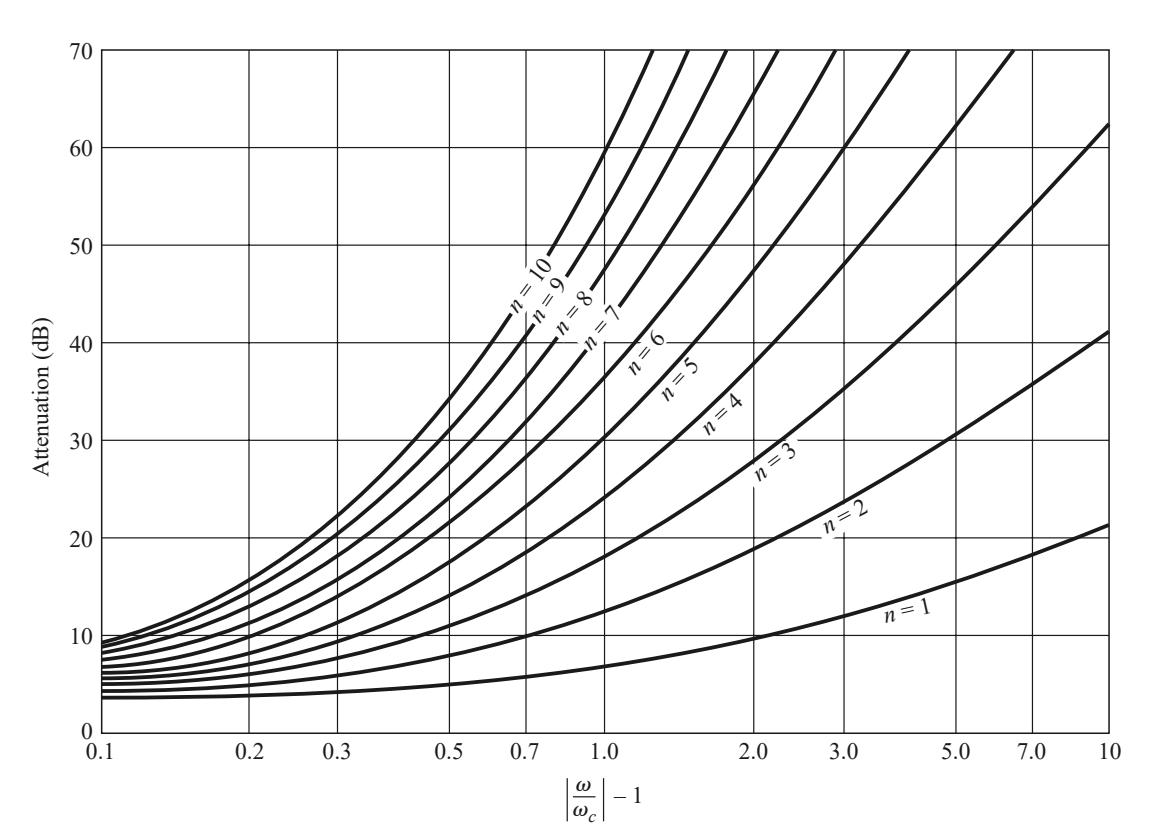
\includegraphics[scale=0.5]{images/butterworth_attenuation_table.png}
    \caption{Attenuation versus normalized frequency for maximally flat filter prototypes.}
    \label{fig:1}
\end{figure}
Once the line closest to the intersecting point is defined using the figure above \ref{fig:1}, we can determine the number of elements ($N$) needed to construct our low-pass, and ultimately band-pass prototype. In doing so, we will use the following table to determine the our element values (i.e., $g_1, g_2,...,g_n$):
\begin{table}[h!]
\centering
\begin{tabular}{| c | c | c | c | c | c | c | c | c | c | c | c |} 
 \hline
 N & $g_1$ & $g_2$ & $g_3$ & $g_4$ & $g_5$ & $g_6$ & $g_7$ & $g_8$ & $g_9$ & $g_{10}$ & $g_{11}$ \\ [0.5ex] 
 \hline
 1 & 2.0000 & 1.0000 & & & & & & & & & \\ 
 \hline
 2 & 1.4142 & 1.4142 & 1.0000 & & & & & & & & \\
 \hline
 3 & 1.0000 & 2.0000 & 1.0000 & 1.0000 & & & & & & & \\
 \hline
 4 & 0.7654 & 1.8478 & 1.8478 & 0.7654 & 1.0000 & & & & & & \\
 \hline
 5 & 0.6180 & 1.6180 & 2.0000 & 1.6180 & 0.6180 & 1.0000 & & & & & \\
 \hline
 6 & 0.5176 & 1.4142 & 1.9318 & 1.9318 & 1.4142 & 0.5176 & 1.0000 & & & & \\
 \hline
 7 & 0.4450 & 1.2470 & 1.8019 & 2.0000 & 1.8019 & 1.2470 & 0.4450 & 1.0000 & & & \\
 \hline
 8 & 0.3902 & 1.1111 & 1.6629 & 1.9615 & 1.9615 & 1.6629 & 1.1111 & 0.3902 & 1.0000 & & \\
 \hline
 9 & 0.3473 & 1.0000 & 1.5321 & 1.8794 & 2.0000 & 1.8794 & 1.5321 & 1.0000 & 0.3473 & 1.000 & \\
 \hline
 10 & 0.3129 & 0.9080 & 1.4142 & 1.7820 & 1.9754 & 1.9754 & 1.7820 & 1.4142 & 0.9080 & 0.3129 & 1.0000 \\
 \hline
\end{tabular}
\caption{Element Values for Maximally Flat Low-Pass Filter Prototypes}
\label{table:2}
\end{table}
\text{ }\\
Given that $N=3$, from the above table \ref{table:2} we can determine the following:
\begin{align*}
    g_1 &= 1.0000 \\
    g_2 &= 2.0000 \\
    g_3 &= 1.0000 \\
\end{align*}
We can now construct our band-pass prototype values for our lumped element equivalent circuit using the values of $g_1$, $g_2$, and $g_3$ as follows:
\begin{align}
    L_1 &= \dfrac{g_1 Z_0}{\omega_0 \Delta} = 21.654 \text{ nH} \\
    C_1 &= \dfrac{\Delta}{g_1 Z_0 \omega_0} = 0.19488 \text{ pF} \\
    L_2 &= \dfrac{Z_0 \Delta}{g_2 \omega_0} = 0.2436 \text{ nH} \\
    C_2 &= \dfrac{g_2}{Z_0 \omega_0 \Delta} = 17.323 \text{ pF} \\
    L_3 &= \dfrac{g_3 Z_0}{\omega_0 \Delta} = 21.654 \text{ nH} \\
    C_3 &= \dfrac{\Delta}{g_3 \omega_0 Z_0} = 0.19488 \text{ pF}
\end{align}
Now we calculate our \textit{Admittance Inverter Constants} using the following formulas:
\begin{align}
    Z_0 J_1 &= \sqrt{\dfrac{\pi \Delta}{2g_1}} \\
    Z_0 J_n &= \dfrac{\pi \Delta}{2\sqrt{g_{n-1}}} \text{ for } n = 2, 3,...,N,\\
    Z_0 J_{N+1} &= \sqrt{\dfrac{\pi \Delta}{2g_N g_{N+1}}}
\end{align}
Then we use the following formulas to calculate our Even-and-Odd-Mode Characteristic Impedances:
\begin{align}
    Z_{0_e} &= Z_0\left[ 1 + Z_0 J_n + (Z_0 J_n)^2 \right]\\
    Z_{0_o} &= Z_0\left[ 1 - Z_0 J_n + (Z_0 J_n)^2 \right]
\end{align}
The resulting schematic and plot of the lumped element equivalent circuit is as follows:
\begin{figure}[h!]
    \centering
    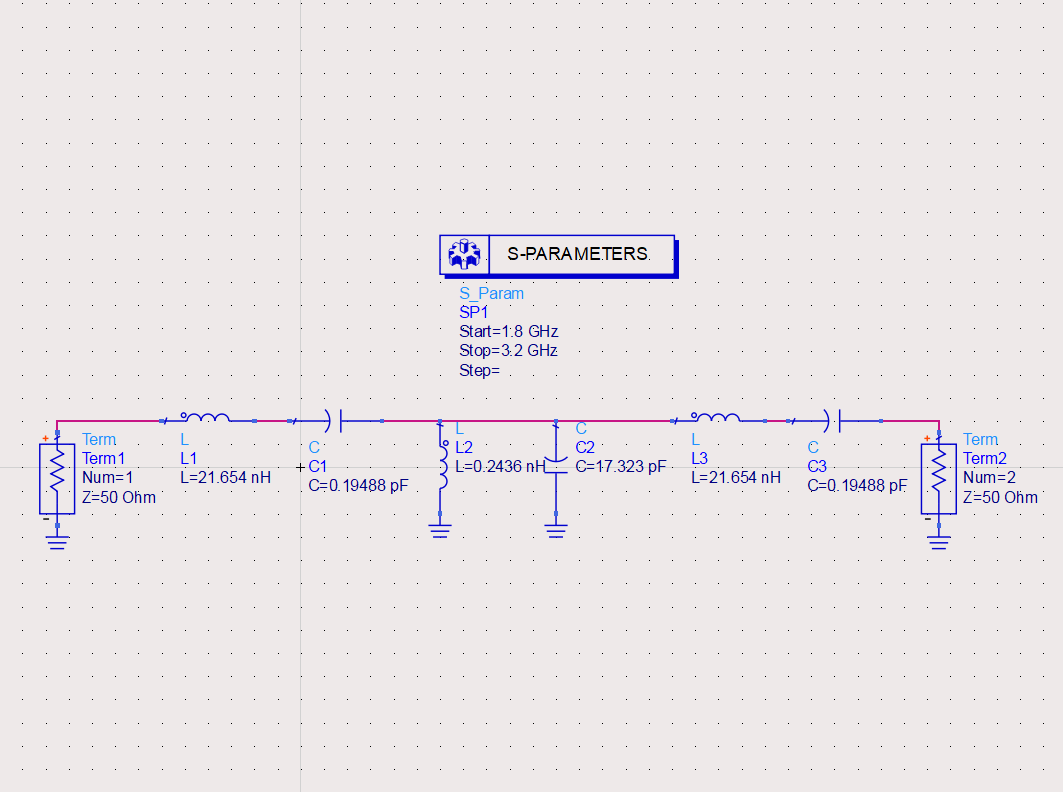
\includegraphics[scale=0.4]{images/butterworth_schematic.png}
    \caption{Butterworth (Maximally Flat) Schematic}
    \label{fig:2}
\end{figure}
\newpage
\begin{figure}[h!]
    \centering
    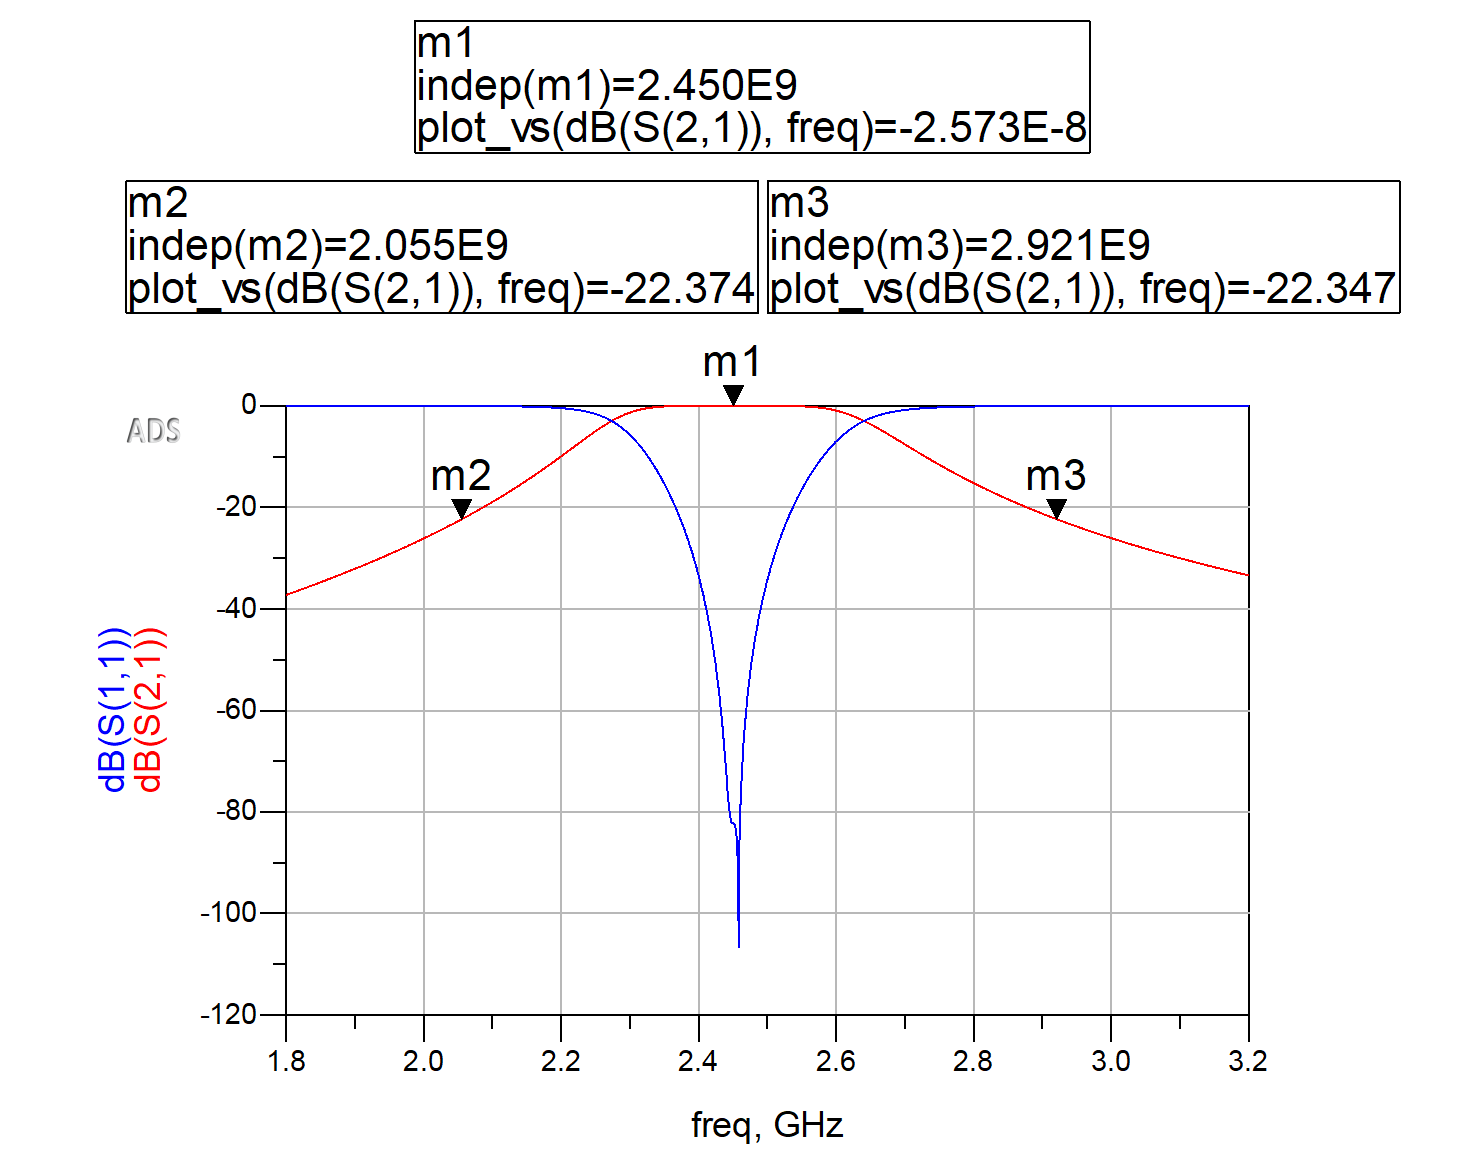
\includegraphics[scale=0.5]{images/butterworth_plot.png}
    \caption{Butterworth (Maximally Flat) Plot}
    \label{fig:3}
\end{figure}

\subsection{Chebyshev 0.5 dB Equal-Ripple Response}
The Chebyshev 0.5 dB Equal-Ripple method provides significantly greater roll-off between the pass-band and stop-band relative to the Butterworth (i.e., Maximally Flat) response, but loses flatness in the pass-band resulting in 0.5 dB \textbf{equal-ripples} across the pass-band.
\subsubsection{Chebyshev 0.5 dB Design Process}
The first step in the design is to determine the number of coupled elements to acquire a desired level of attenuation at a specific frequency relative to the center frequency of the desired signal. This is accomplished by determining a normalized frequency as follows:
\begin{equation}
    \omega \leftarrow \dfrac{\omega_0}{\omega_2 - \omega_1} \left( \dfrac{\omega}{\omega_0} - \dfrac{\omega_0}{\omega} \right) = \dfrac{1}{\Delta} \left( \dfrac{\omega}{\omega_0} - \dfrac{\omega_0}{\omega} \right)
\end{equation}
where,\\
\begin{equation}
    \Delta = \dfrac{\omega_2 - \omega_1}{\omega_0}
\end{equation}
is the fractional bandwidth of the passband. The center frequency, $\omega_0$, could be chosen as the arithmetic mean of $\omega_1$ and $\omega_2$, but the equations are simpler if it is chosen as the geometric mean:
\begin{equation}
    \omega_0 = \sqrt{\omega_1 \omega_2}
\end{equation}
Then the scale of the horizontal scale of Figure 8.27 is:
\begin{equation}
    \left| \dfrac{\omega}{\omega_c} \right| - 1
\end{equation}
\textbf{It is important to note that $\omega_c$ is equal to 1 in this normalized form.}\cite{Pozar}\\
\textbf{ }\\
Given the criteria defined for \textbf{all} of our designs, the resulting value given our normalized frequency is: $1.3566$\\
\text{ }\\
Now, using the value calculated above (1.3566), we use the figure to determine the number of elements to acquire an attenuation of 20 dB by finding the intersection of $1.3566$ on the x-axis, and the line consistent with the y-axis value of 20 dB attenuation:
\newpage
\begin{figure}[h!]
    \centering
    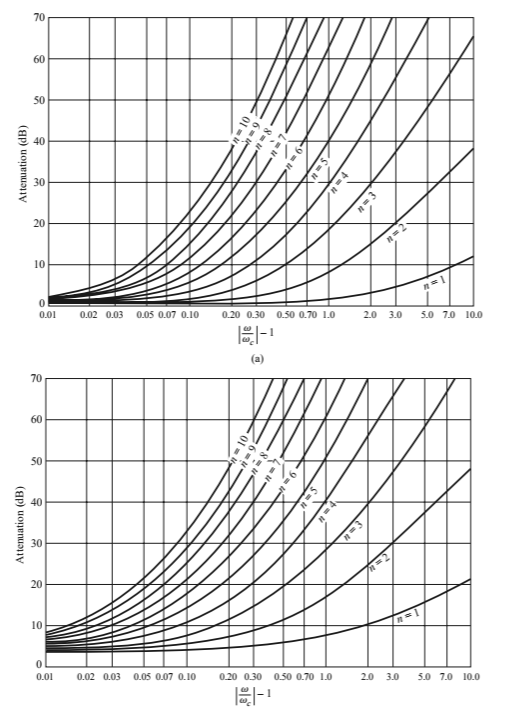
\includegraphics[scale=1.0]{images/chebyshev_attenuation_table.png}
    \caption{Attenuation versus normalized frequency for 0.5 and 3 dB Equal-Ripple (Chebyshev) filter prototypes}
    \label{fig:4}
\end{figure}
Once the line closest to the intersecting point is defined using the figure above \ref{fig:1}, we can determine the number of elements ($N$) needed to construct our low-pass, and ultimately band-pass prototype. In doing so, we will use the following table to determine the our element values (i.e., $g_1, g_2,...,g_n$):
\begin{table}[h!]
\centering
\begin{tabular}{| c | c | c | c | c | c | c | c | c | c | c | c |} 
 \hline
 N & $g_1$ & $g_2$ & $g_3$ & $g_4$ & $g_5$ & $g_6$ & $g_7$ & $g_8$ & $g_9$ & $g_{10}$ & $g_{11}$ \\ [0.5ex] 
 \hline
 1 & 0.6986 & 1.0000 & & & & & & & & & \\ 
 \hline
 2 & 1.4029 & 0.7071 & 1.9841 & & & & & & & & \\
 \hline
 3 & 1.5963 & 1.0967 & 1.5963 & 1.0000 & & & & & & & \\
 \hline
 4 & 1.6703 & 1.1926 & 2.3661 & 0.8419 & 1.9841 & & & & & & \\
 \hline
 5 & 1.7058 & 1.2296 & 2.5408 & 1.2296 & 1.7058 & 1.0000 & & & & & \\
 \hline
 6 & 1.7254 & 1.2479 & 2.6064 & 1.3137 & 2.4748 & 0.8696 & 1.9841 & & & & \\
 \hline
 7 & 1.7372 & 1.2583 & 2.6381 & 1.3444 & 2.6381 & 1.2583 & 1.7372 & 1.0000 & & & \\
 \hline
 8 & 1.7451 & 1.2647 & 2.6564 & 1.3590 & 2.6964 & 1.3389 & 2.5093 & 0.8796 & 1.9841 & & \\
 \hline
 9 & 1.7504 & 1.2690 & 2.6678 & 1.3673 & 2.7239 & 1.3673 & 2.6678 & 1.2690 & 1.7504 & 1.000 & \\
 \hline
 10 & 1.7543 & 1.2721 & 2.6754 & 1.3725 & 2.7392 & 1.3806 & 2.7231 & 1.3485 & 2.5239 & 0.8842 & 1.9841 \\
 \hline
\end{tabular}
\caption{Element Values for 0.5 dB Equal-Ripple Low-Pass Filter Prototypes}
\label{table:3}
\end{table}
\text{ }\\
Given that $N=3$, from the above table \ref{table:2} we can determine the following:
\begin{align*}
    g_1 &= 1.5963 \\
    g_2 &= 1.0967 \\
    g_3 &= 1.5963 \\
\end{align*}
We can now construct our band-pass prototype values for our lumped element equivalent circuit using the values of $g_1$, $g_2$, and $g_3$ as follows:
\begin{align}
    L_1 &= \dfrac{g_1 Z_0}{\omega_0 \Delta} = 33.341 \text{ nH} \\
    C_1 &= \dfrac{\Delta}{g_1 Z_0 \omega_0} = 0.11776 \text{ pF} \\
    L_2 &= \dfrac{Z_0 \Delta}{g_2 \omega_0} = 42.851 \text{ nH} \\
    C_2 &= \dfrac{g_2}{Z_0 \omega_0 \Delta} = 9.1625 \text{ pF} \\
    L_3 &= \dfrac{g_3 Z_0}{\omega_0 \Delta} = 33.341 \text{ nH} \\
    C_3 &= \dfrac{\Delta}{g_3 \omega_0 Z_0} = 0.11776 \text{ pF}
\end{align}
Now we calculate our \textit{Admittance Inverter Constants} using the following formulas:
\begin{align}
    Z_0 J_1 &= \sqrt{\dfrac{\pi \Delta}{2g_1}} \\
    Z_0 J_n &= \dfrac{\pi \Delta}{2\sqrt{g_{n-1}}} \text{ for } n = 2, 3,...,N,\\
    Z_0 J_{N+1} &= \sqrt{\dfrac{\pi \Delta}{2g_N g_{N+1}}}
\end{align}
Then we use the following formulas to calculate our Even-and-Odd-Mode Characteristic Impedances:
\begin{align}
    Z_{0_e} &= Z_0\left[ 1 + Z_0 J_n + (Z_0 J_n)^2 \right]\\
    Z_{0_o} &= Z_0\left[ 1 - Z_0 J_n + (Z_0 J_n)^2 \right]
\end{align}
The resulting schematic and plot of the lumped element equivalent circuit is as follows:
\begin{figure}[h!]
    \centering
    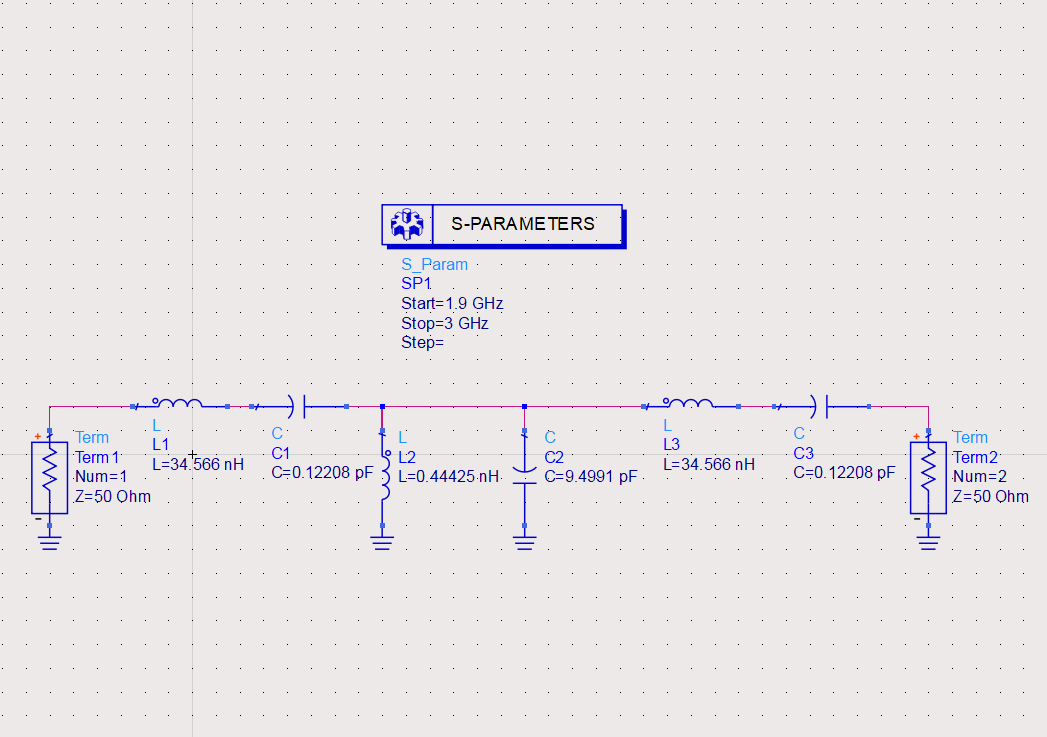
\includegraphics[scale=0.5]{images/chebyshev_0pt5_schematic.png}
    \caption{Chebyshev 0.5 Equal-Ripple Schematic}
    \label{fig:5}
\end{figure}
\begin{figure}
    \centering
    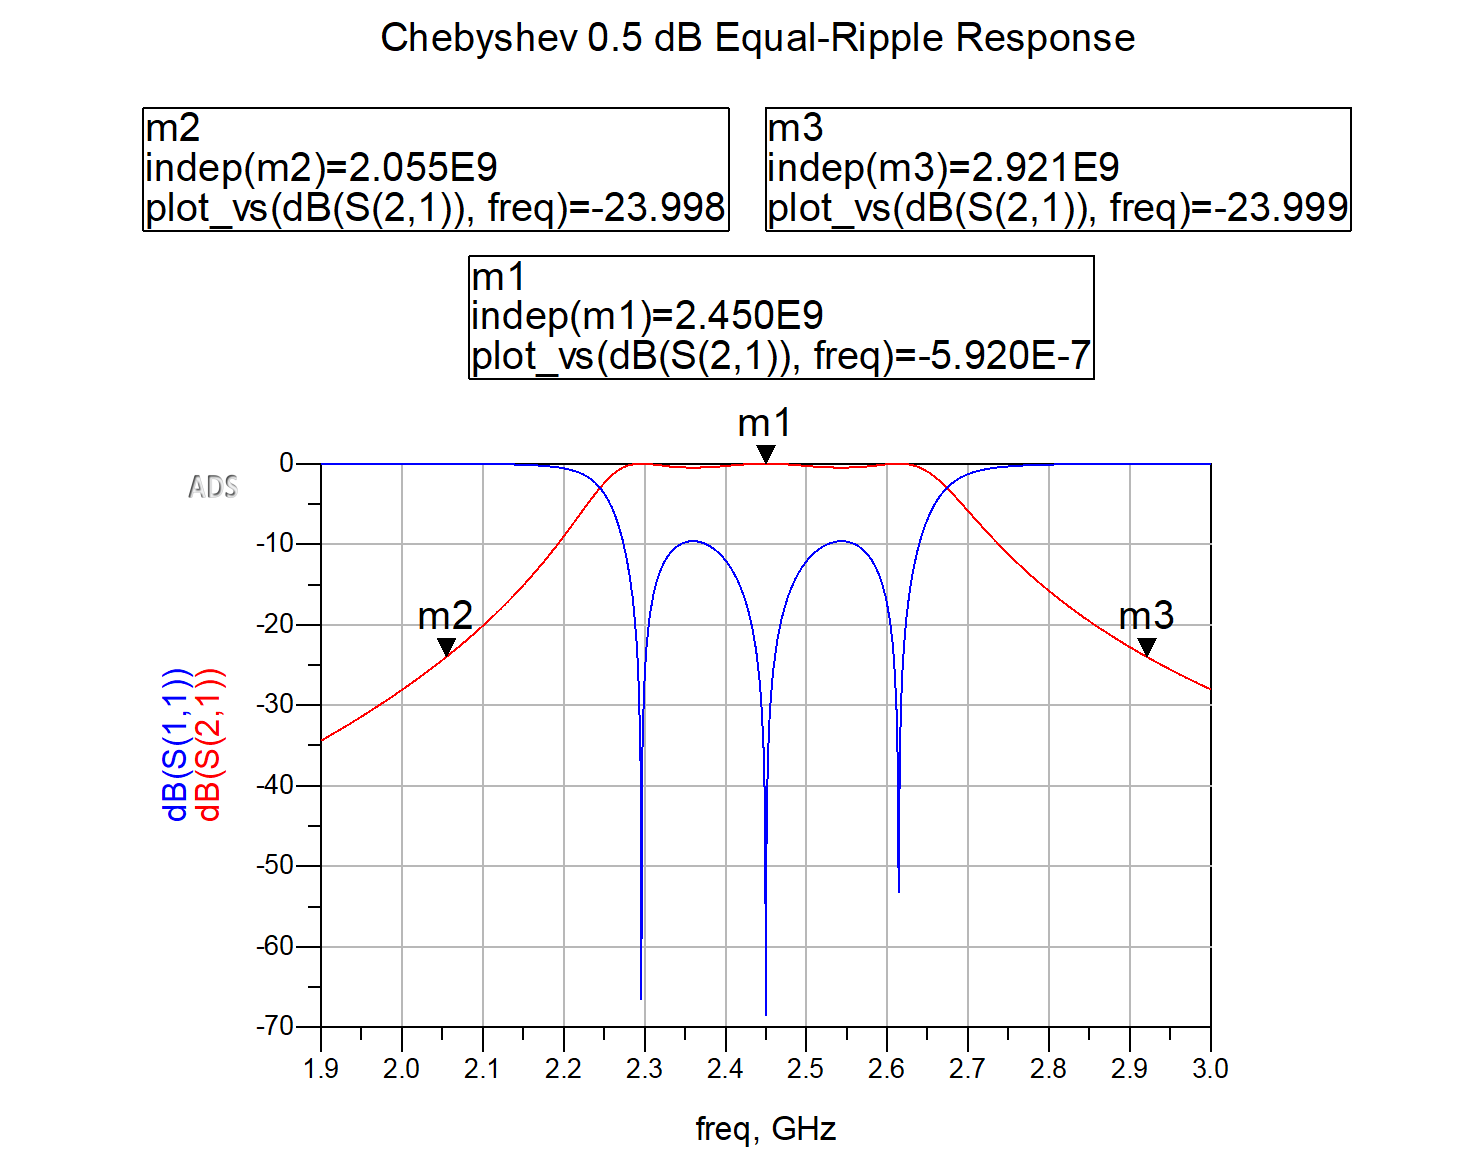
\includegraphics[scale=0.5]{images/chebyshev_0pt5_plot.png}
    \caption{Chebyshev 0.5 Equal-Ripple Plot}
    \label{fig:6}
\end{figure}
\newpage

\subsection{Chebyshev 3 dB Equal-Ripple Response}
The Chebyshev 3 dB Equal-Ripple method provides significantly greater roll-off between the pass-band and stop-band relative to the Butterworth (i.e., Maximally Flat) response, but loses flatness in the pass-band resulting in 3 dB \textbf{equal-ripples} across the pass-band.
\subsubsection{Chebyshev 3 dB Equal-Ripple Design Process}
The first step in the design is to determine the number of coupled elements to acquire a desired level of attenuation at a specific frequency relative to the center frequency of the desired signal. This is accomplished by determining a normalized frequency as follows:
\begin{equation}
    \omega \leftarrow \dfrac{\omega_0}{\omega_2 - \omega_1} \left( \dfrac{\omega}{\omega_0} - \dfrac{\omega_0}{\omega} \right) = \dfrac{1}{\Delta} \left( \dfrac{\omega}{\omega_0} - \dfrac{\omega_0}{\omega} \right)
\end{equation}
where,\\
\begin{equation}
    \Delta = \dfrac{\omega_2 - \omega_1}{\omega_0}
\end{equation}
is the fractional bandwidth of the passband. The center frequency, $\omega_0$, could be chosen as the arithmetic mean of $\omega_1$ and $\omega_2$, but the equations are simpler if it is chosen as the geometric mean:
\begin{equation}
    \omega_0 = \sqrt{\omega_1 \omega_2}
\end{equation}
Then the scale of the horizontal scale of Figure 8.27 is:
\begin{equation}
    \left| \dfrac{\omega}{\omega_c} \right| - 1
\end{equation}
\textbf{It is important to note that $\omega_c$ is equal to 1 in this normalized form.}\cite{Pozar}\\
\textbf{ }\\
Given the criteria defined for \textbf{all} of our designs, the resulting value given our normalized frequency is: $1.3566$\\
\text{ }\\
Now, using the value calculated above (1.3566), we use the figure to determine the number of elements to acquire an attenuation of 20 dB by finding the intersection of $1.3566$ on the x-axis, and the line consistent with the y-axis value of 20 dB attenuation:
\newpage
\begin{figure}[h!]
    \centering
    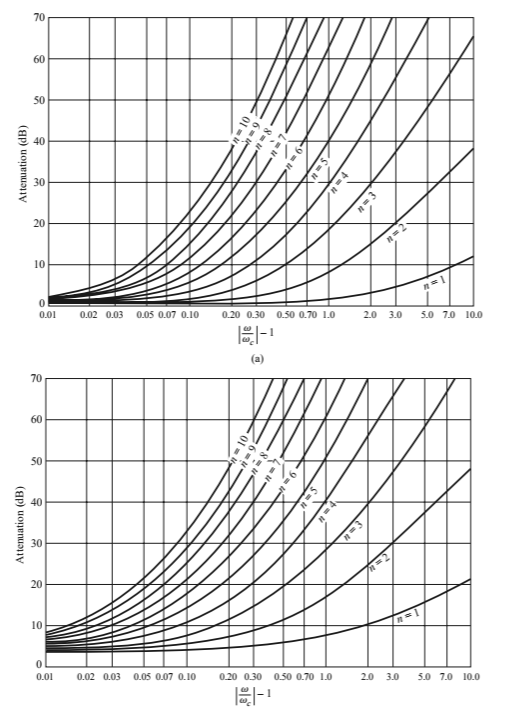
\includegraphics[scale=1.0]{images/chebyshev_attenuation_table.png}
    \caption{Attenuation versus normalized frequency for 0.5 and 3 dB Equal-Ripple (Chebyshev) filter prototypes}
    \label{fig:7}
\end{figure}
Once the line closest to the intersecting point is defined using the figure above \ref{fig:1}, we can determine the number of elements ($N$) needed to construct our low-pass, and ultimately band-pass prototype. In doing so, we will use the following table to determine the our element values (i.e., $g_1, g_2,...,g_n$):
\begin{table}[h!]
\centering
\begin{tabular}{| c | c | c | c | c | c | c | c | c | c | c | c |} 
 \hline
 N & $g_1$ & $g_2$ & $g_3$ & $g_4$ & $g_5$ & $g_6$ & $g_7$ & $g_8$ & $g_9$ & $g_{10}$ & $g_{11}$ \\ [0.5ex] 
 \hline
 1 & 1.9953 & 1.0000 & & & & & & & & & \\ 
 \hline
 2 & 3.1013 & 0.5339 & 5.8095 & & & & & & & & \\
 \hline
 3 & 3.3487 & 0.7117 & 3.3487 & 1.0000 & & & & & & & \\
 \hline
 4 & 3.4389 & 0.7483 & 4.3471 & 0.5920 & 5.8095 & & & & & & \\
 \hline
 5 & 3.4817 & 0.7618 & 4.5381 & 0.7618 & 3.4817 & 1.0000 & & & & & \\
 \hline
 6 & 3.5045 & 0.7685 & 4.6061 & 0.7929 & 4.4641 & 0.6033 & 5.8095 & & & & \\
 \hline
 7 & 3.5182 & 0.7723 & 4.6386 & 0.8039 & 4.6386 & 0.7723 & 3.5182 & 1.0000 & & & \\
 \hline
 8 & 3.5277 & 0.7745 & 4.6575 & 0.8089 & 4.6990 & 0.8018 & 4.4990 & 0.6073 & 5.8095 & & \\
 \hline
 9 & 3.5340 & 0.7760 & 4.6692 & 0.8118 & 4.7272 & 0.8118 & 4.6692 & 0.7760 & 3.5340 & 1.0000 & \\
 \hline
 10 & 3.5384 & 0.7771 & 4.6768 & 0.8136 & 4.7425 & 0.8164 & 4.7260 & 0.8051 & 4.5142 & 0.6091 & 5.8095 \\
 \hline
\end{tabular}
\caption{Element Values for 3 dB Equal-Ripple Low-Pass Filter Prototypes}
\label{table:4}
\end{table}
Given that $N=3$, from the above table \ref{table:2} we can determine the following:
\begin{align*}
    g_1 &= 3.3487 \\
    g_2 &= 0.7117 \\
    g_3 &= 3.3487 \\
\end{align*}
We can now construct our band-pass prototype values for our lumped element equivalent circuit using the values of $g_1$, $g_2$, and $g_3$ as follows:
\begin{align}
    L_1 &= \dfrac{g_1 Z_0}{\omega_0 \Delta} = 72.512 \text{ nH} \\
    C_1 &= \dfrac{\Delta}{g_1 Z_0 \omega_0} = 0.058197 \text{ pF} \\
    L_2 &= \dfrac{Z_0 \Delta}{g_2 \omega_0} = 0.68457 \text{ nH} \\
    C_2 &= \dfrac{g_2}{Z_0 \omega_0 \Delta} = 6.1644 \text{ pF} \\
    L_3 &= \dfrac{g_3 Z_0}{\omega_0 \Delta} = 34.566 \text{ nH} \\
    C_3 &= \dfrac{\Delta}{g_3 \omega_0 Z_0} = 0.12208 \text{ pF}
\end{align}
Now we calculate our \textit{Admittance Inverter Constants} using the following formulas:
\begin{align}
    Z_0 J_1 &= \sqrt{\dfrac{\pi \Delta}{2g_1}} \\
    Z_0 J_n &= \dfrac{\pi \Delta}{2\sqrt{g_{n-1}}} \text{ for } n = 2, 3,...,N,\\
    Z_0 J_{N+1} &= \sqrt{\dfrac{\pi \Delta}{2g_N g_{N+1}}}
\end{align}
Then we use the following formulas to calculate our Even-and-Odd-Mode Characteristic Impedances:
\begin{align}
    Z_{0_e} &= Z_0\left[ 1 + Z_0 J_n + (Z_0 J_n)^2 \right]\\
    Z_{0_o} &= Z_0\left[ 1 - Z_0 J_n + (Z_0 J_n)^2 \right]
\end{align}
The resulting schematic and plot of the lumped element equivalent circuit is as follows:
\begin{figure}[h!]
    \centering
    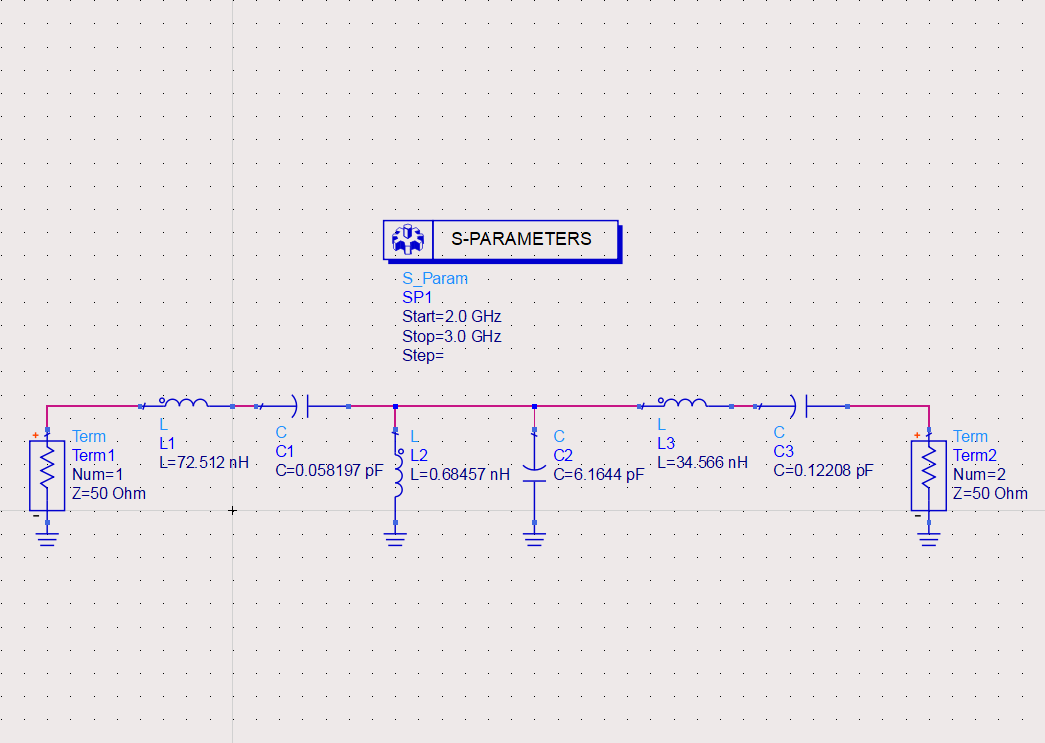
\includegraphics[scale=0.5]{images/chebyshev_3pt0_schematic.png}
    \caption{Chebyshev 3 dB Equal-Ripple Schematic}
    \label{fig:8}
\end{figure}
\begin{figure}[h!]
    \centering
    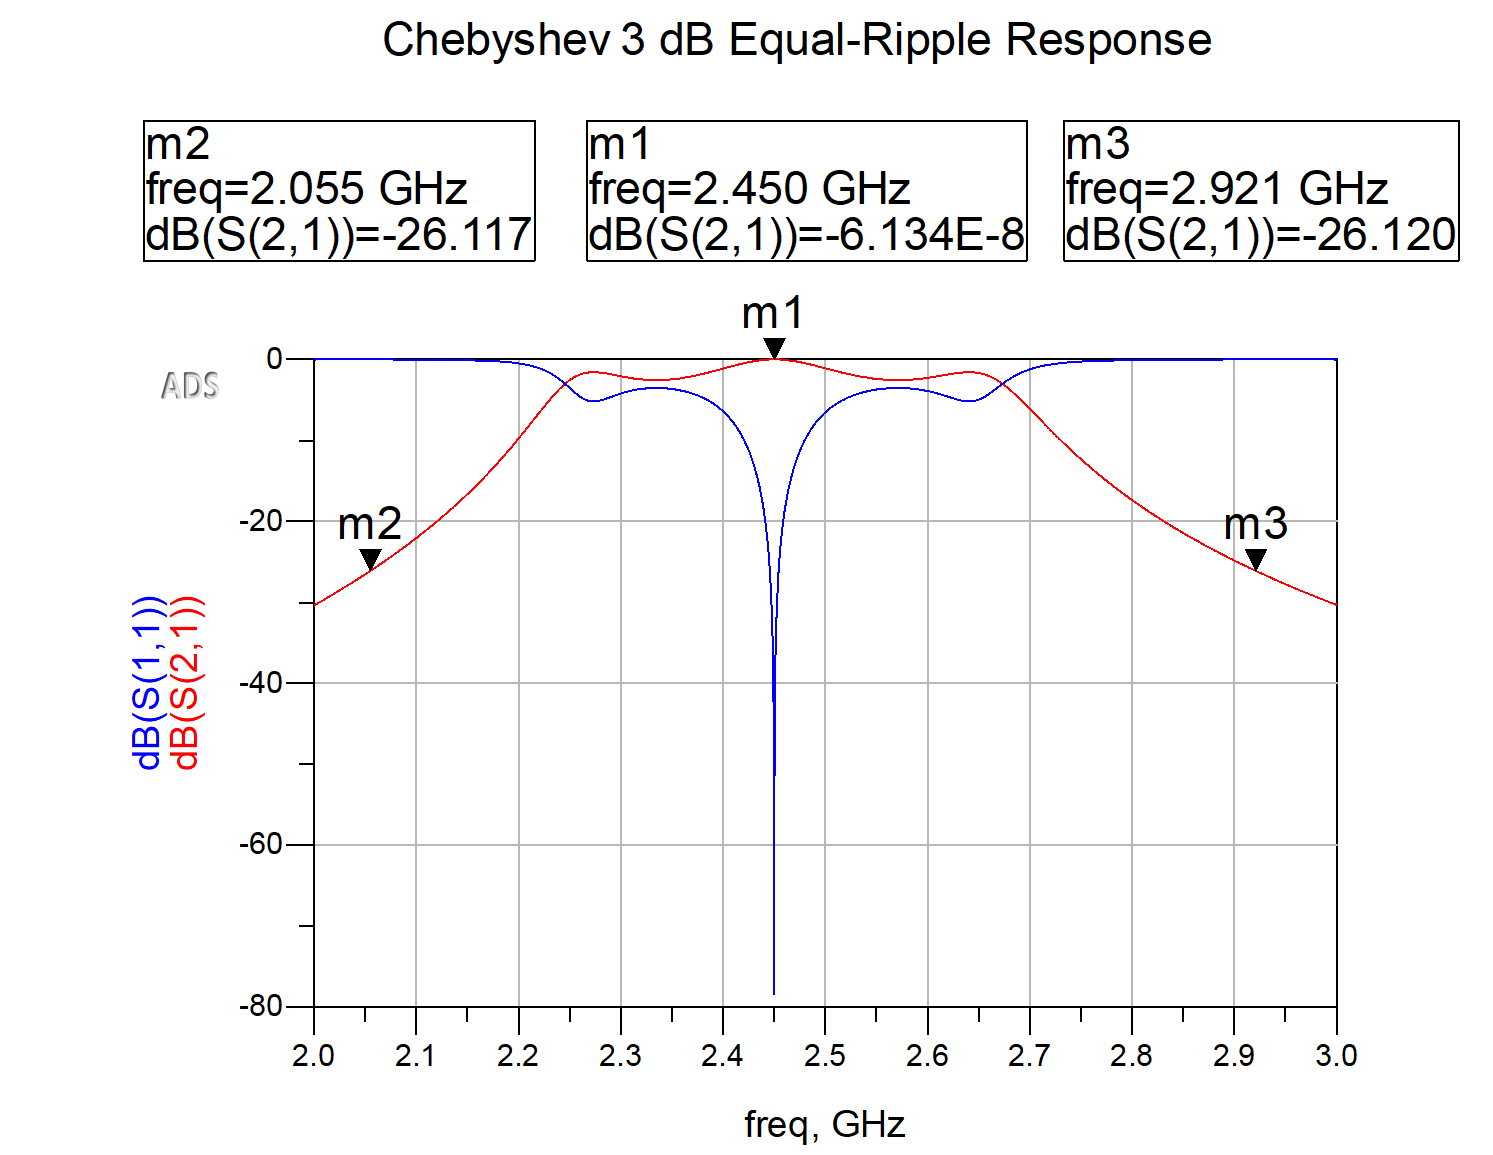
\includegraphics[scale=0.5]{images/chebyshev_3pt0_plot.png}
    \caption{Chebyshev 3 dB Equal-Ripple Plot}
    \label{fig:9}
\end{figure}

\newpage
\section{Coupled Microstrip Line ADS Model}
The following are results from utilizing the MCLIN and MCFIL components individually, and then compared with one another:
\begin{figure}[h!]
    \centering
    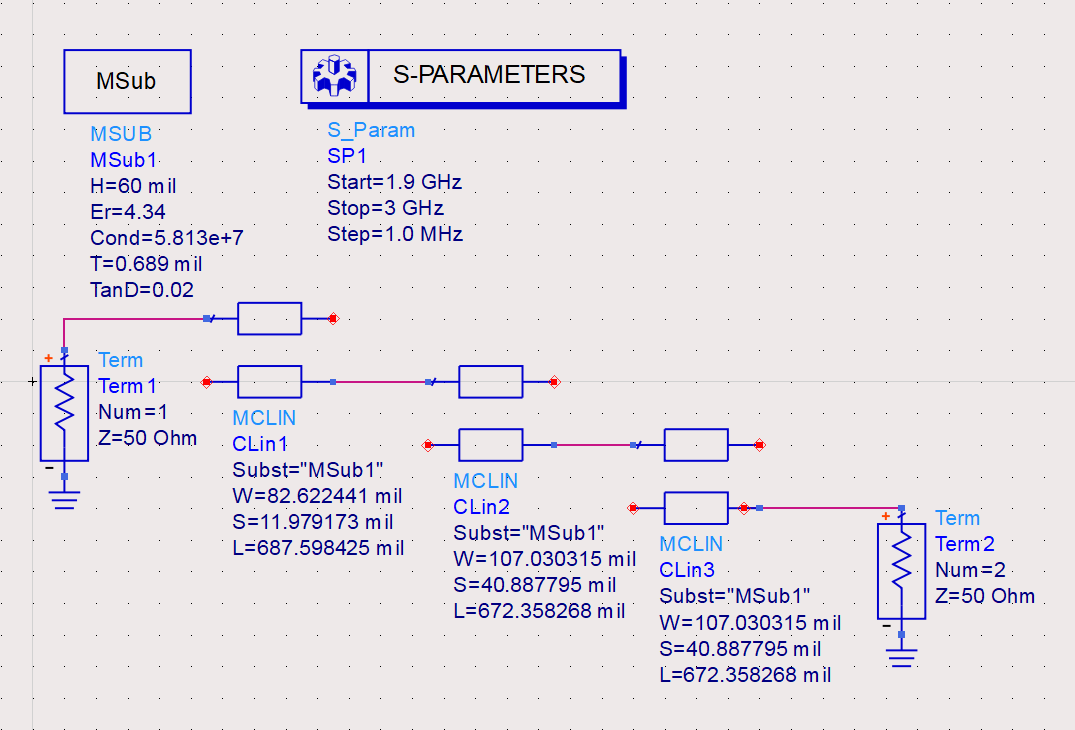
\includegraphics[scale=0.4]{images/mclin_schematic.png}
    \caption{MCLIN Schematic}
    \label{fig:10}
\end{figure}
\begin{figure}[h!]
    \centering
    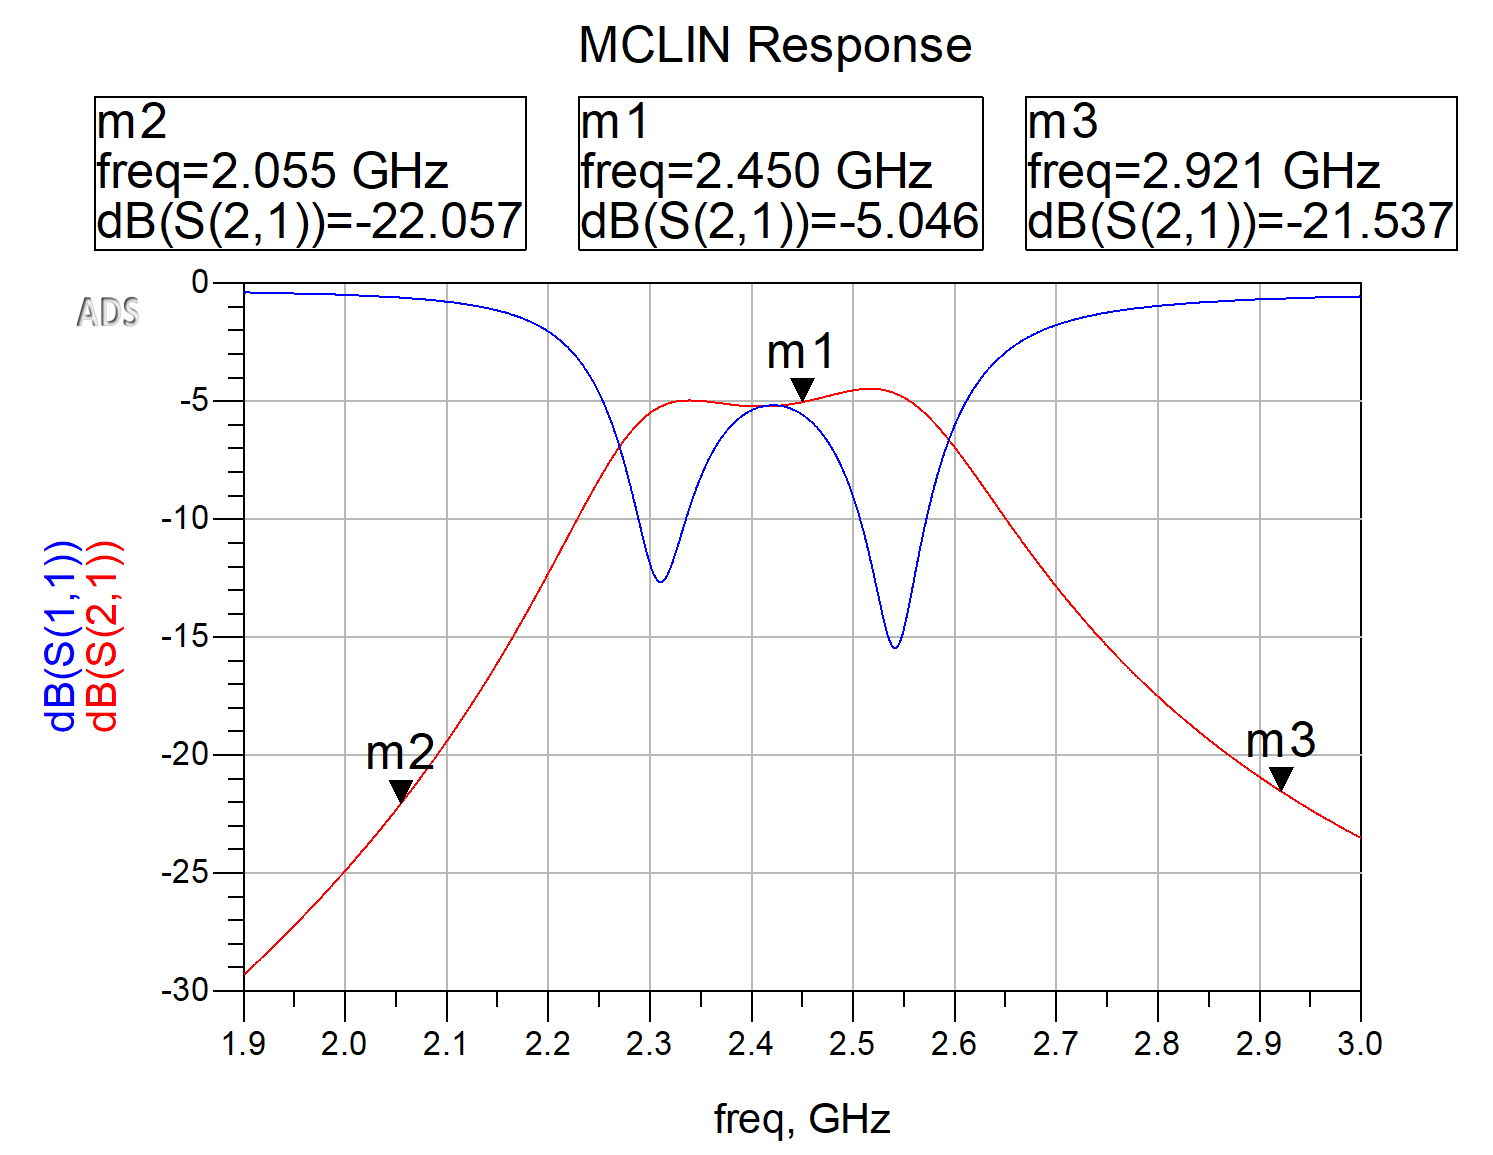
\includegraphics[scale=0.3]{images/mclin_plot.png}
    \caption{MCLIN Plot}
    \label{fig:11}
\end{figure}
\begin{figure}[h!]
    \centering
    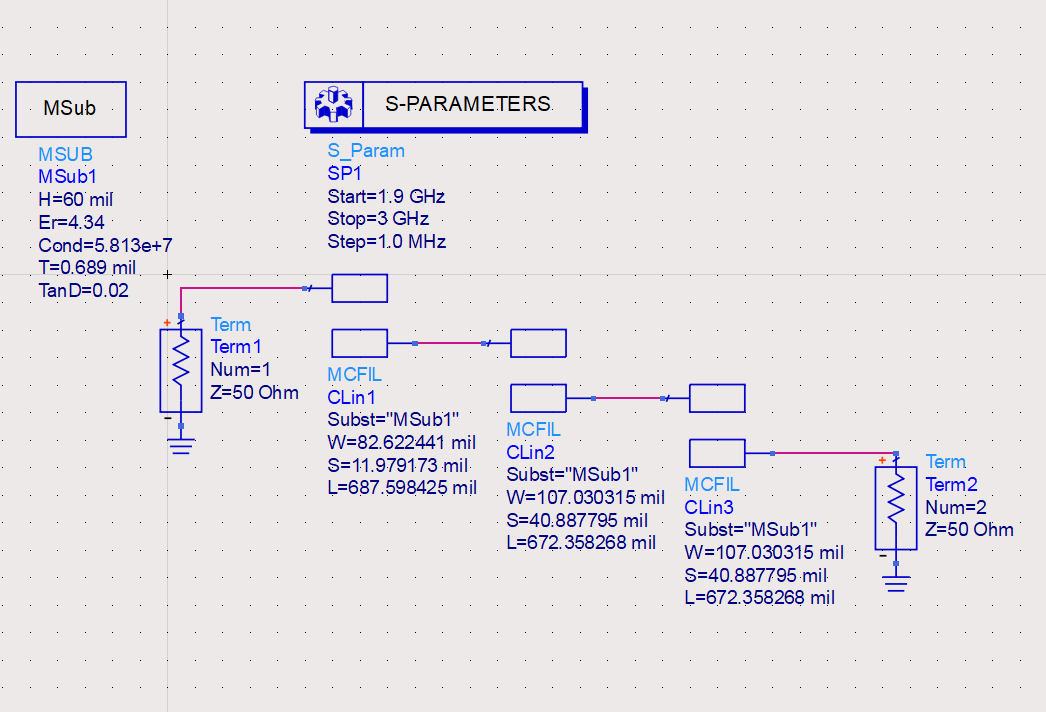
\includegraphics[scale=0.4]{images/mcfil_schematic.png}
    \caption{MCFIL Schematic}
    \label{fig:12}
\end{figure}
\begin{figure}[h!]
    \centering
    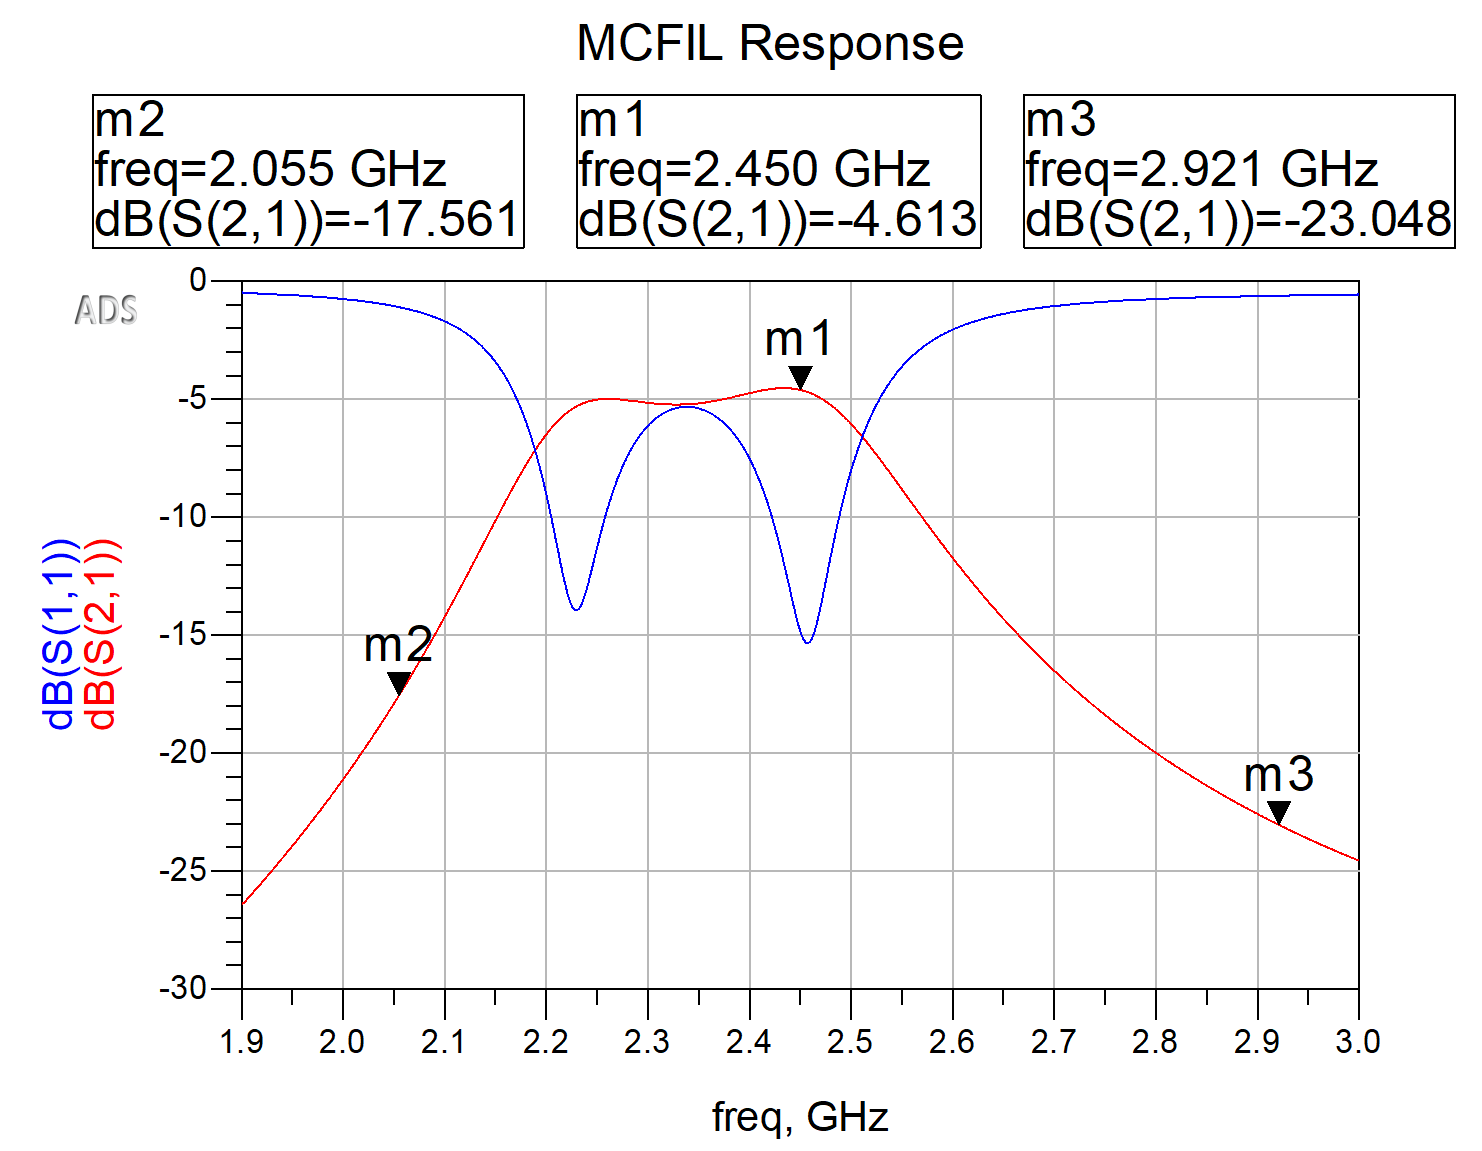
\includegraphics[scale=0.3]{images/mcfil_plot.png}
    \caption{MCFIL Plot}
    \label{fig:13}
\end{figure}


\section{Conclusions}
After analyzing multiple variations of models in ADS it was determined the most accurate model in analysis was using the microstrip coupled line (MCLIN) elements. When analyzed using the MCFIL components the higher frequency stop band roll-off demonstrated greater deviation and was ultimately less accurate.\\
\text{ }\\
It is also clear there are instances where a Butterworth filter would be more advantageous despite the diminished roll-off due to the frequency stability (flatness) in the pass-band, but in most circumstances the 0.5 dB Equal-Ripple Chebyshev would be a more ideal option.\\
\text{  }\\

Also, the 3 dB Equal-Ripple demonstrated the least performance due to the significance of the ripples in the pass-band even with the improved roll-off relative to the Butterworth filter.\\
\text{ }\\ 

Lastly, my design had a critical flaw in the layout design with the layout not leaving enough edge space to ground both SMA pins to the ground plane. This ultimately led to extremely poor performance when analyzed through the FieldFox VNA.
\newpage

\begin{figure}[h!]
    \centering
    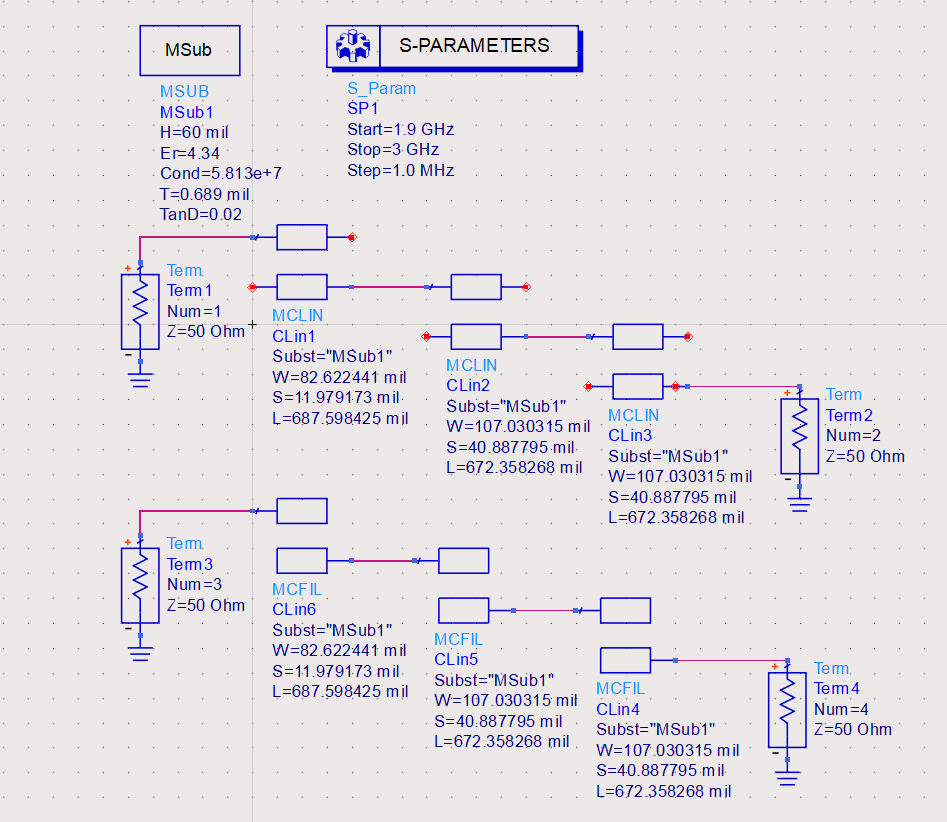
\includegraphics[scale=0.4]{images/mcfil_vs_mclin_schematic.png}
    \caption{MCLIN vs. MCFIL Schematic}
    \label{fig:14}
\end{figure}
\begin{figure}[h!]
    \centering
    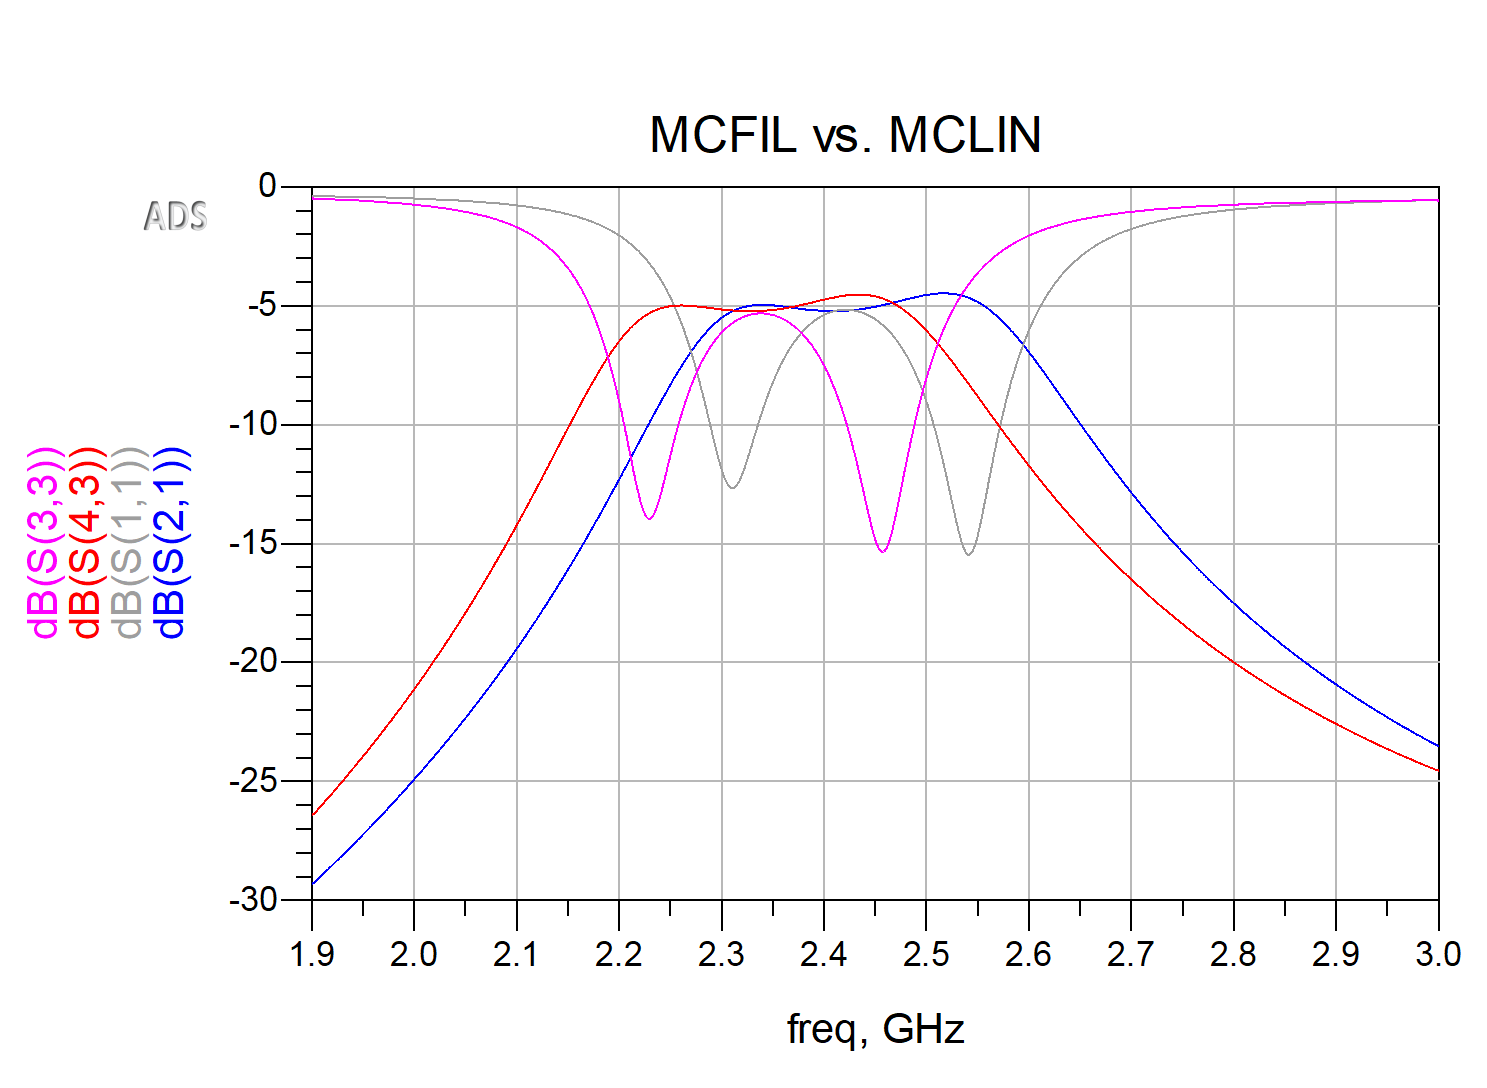
\includegraphics[scale=0.25]{images/mcfil_vs_mclin_plot.png}
    \caption{MCLIN vs. MCFIL Plot}
    \label{fig:15}
\end{figure}
\begin{figure}[h!]
    \centering
    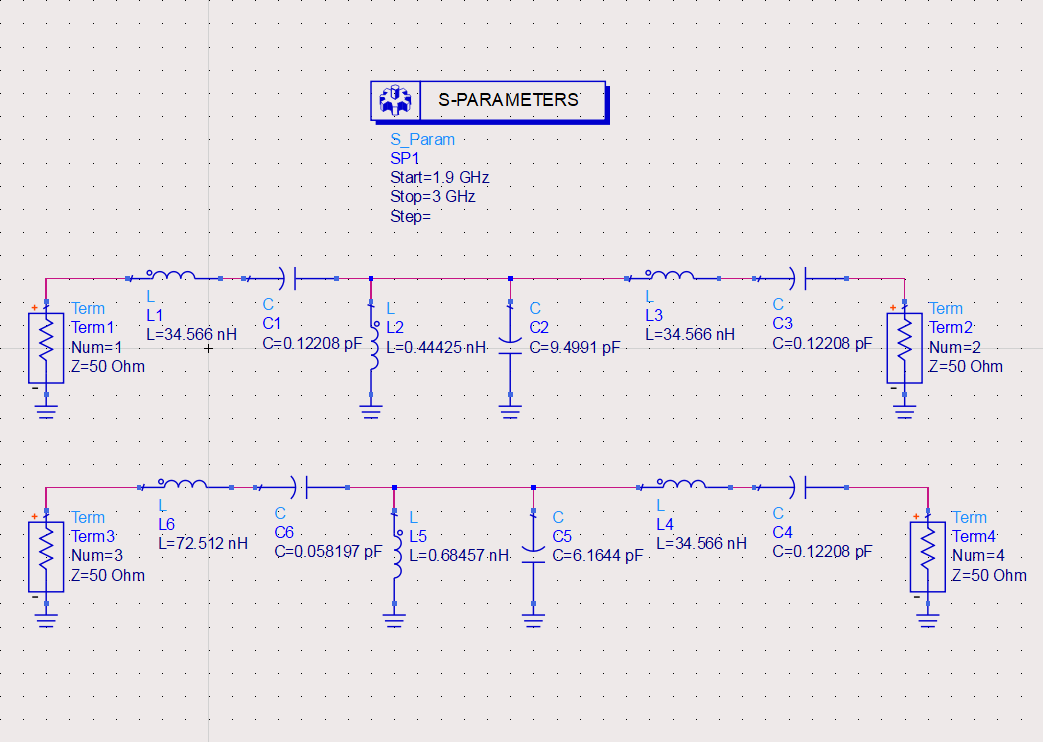
\includegraphics[scale=0.4]{images/chebyshev_0pt5_vs_3pt0_schematic.png}
    \caption{Chebyshev 0.5 vs. 3 dB Schematic}
    \label{fig:16}
\end{figure}
\begin{figure}[h!]
    \centering
    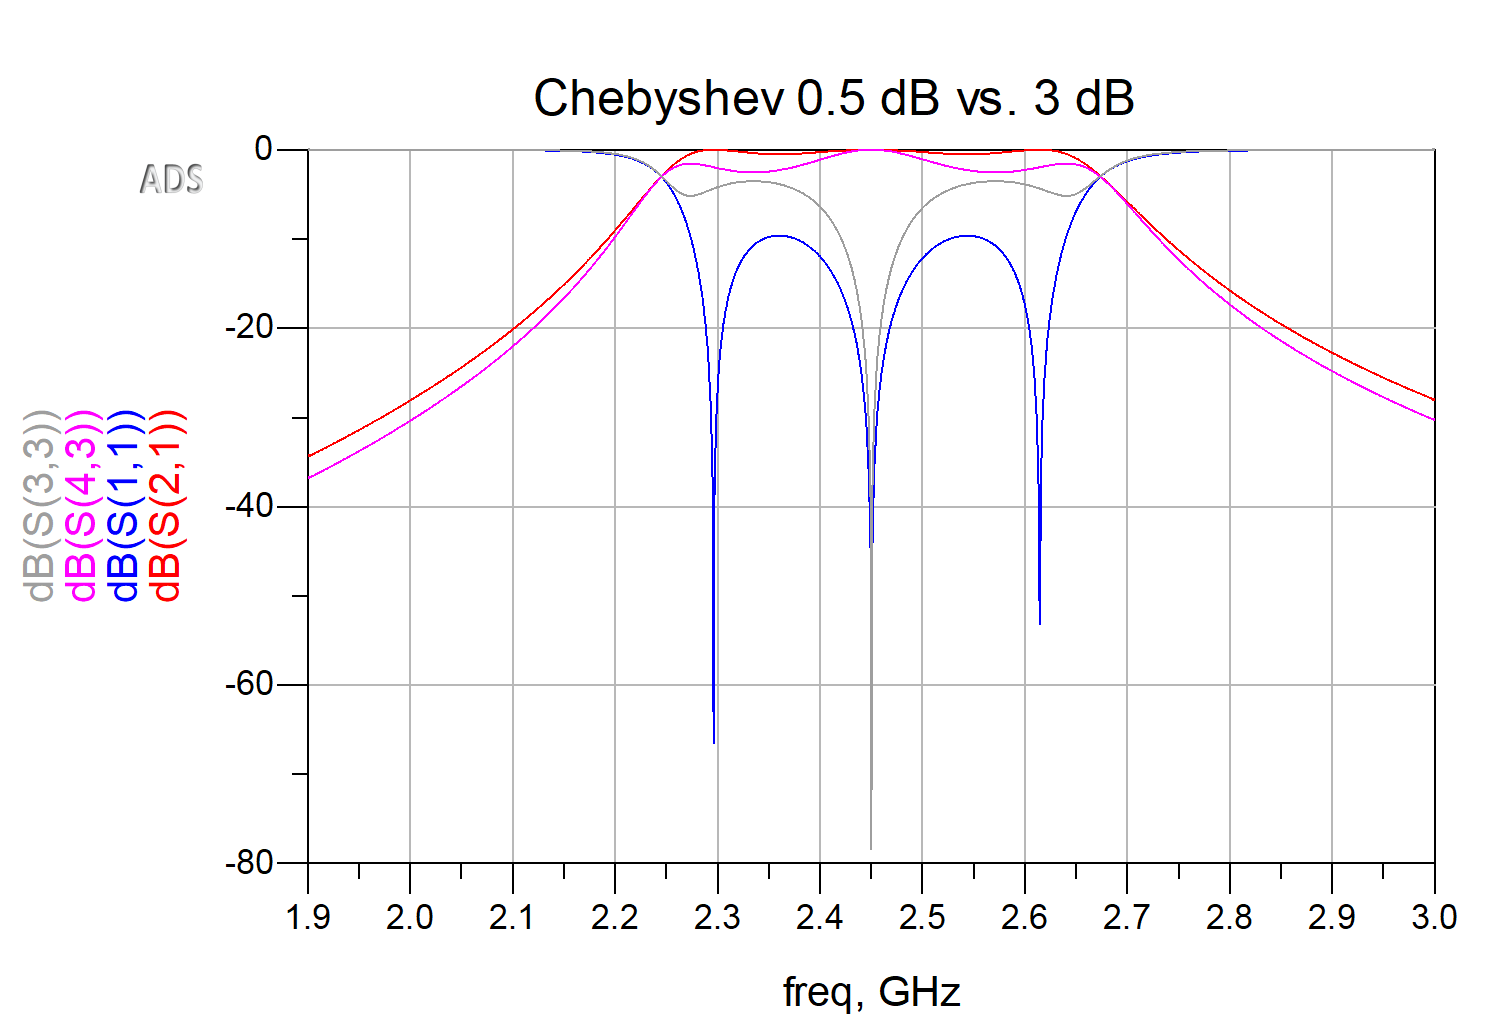
\includegraphics[scale=0.3]{images/chebyshev_0pt5_vs_3pt0_plot.png}
    \caption{Chebyshev 0.5 vs. 3 dB Plot}
    \label{fig:17}
\end{figure}
\begin{figure}[h!]
    \centering
    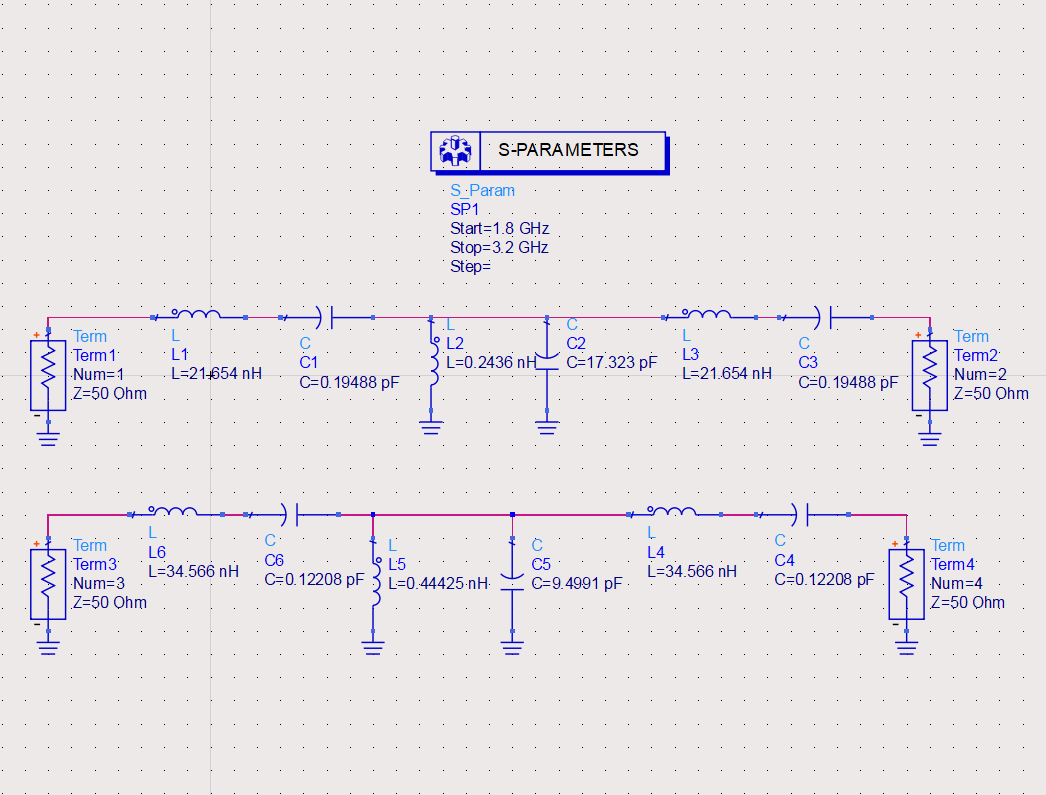
\includegraphics[scale=0.4]{images/butterworth_vs_chebyshev0pt5_schematic.png}
    \caption{Butterworth vs. 0.5 dB Chebyshev Schematic}
    \label{fig:18}
\end{figure}
\begin{figure}[h!]
    \centering
    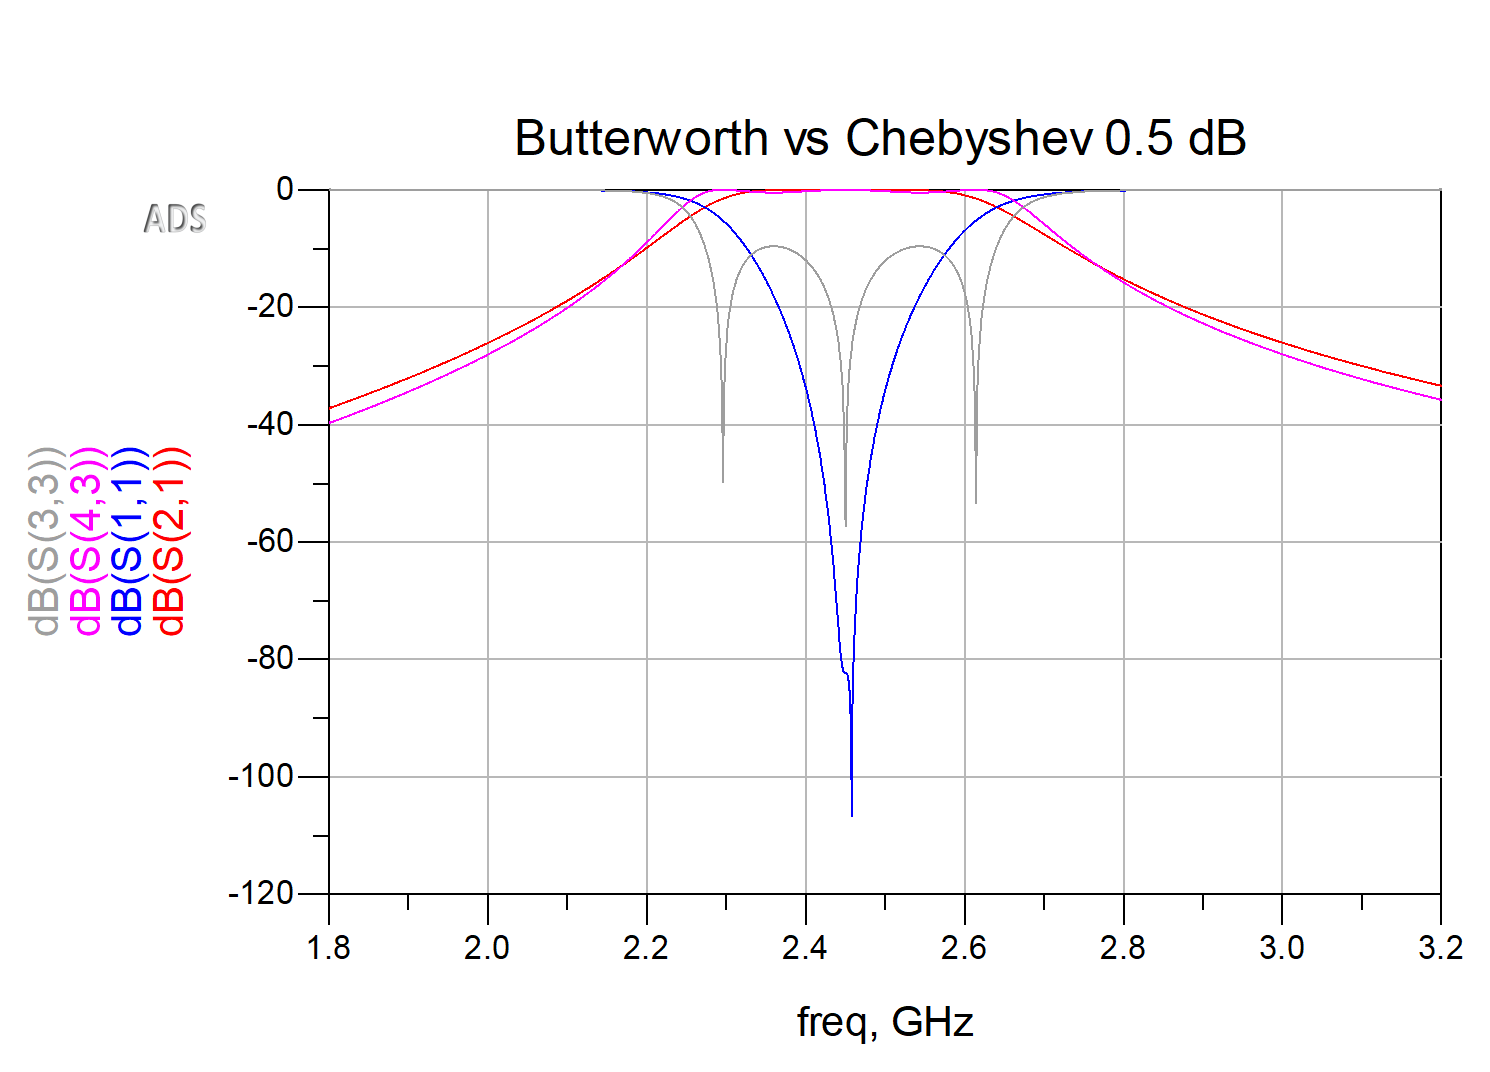
\includegraphics[scale=0.3]{images/butterworth_vs_chebyshev0pt5_plot.png}
    \caption{Butterworth vs. 0.5 dB Chebyshev Plot}
    \label{fig:19}
\end{figure}
\begin{figure}[h!]
    \centering
    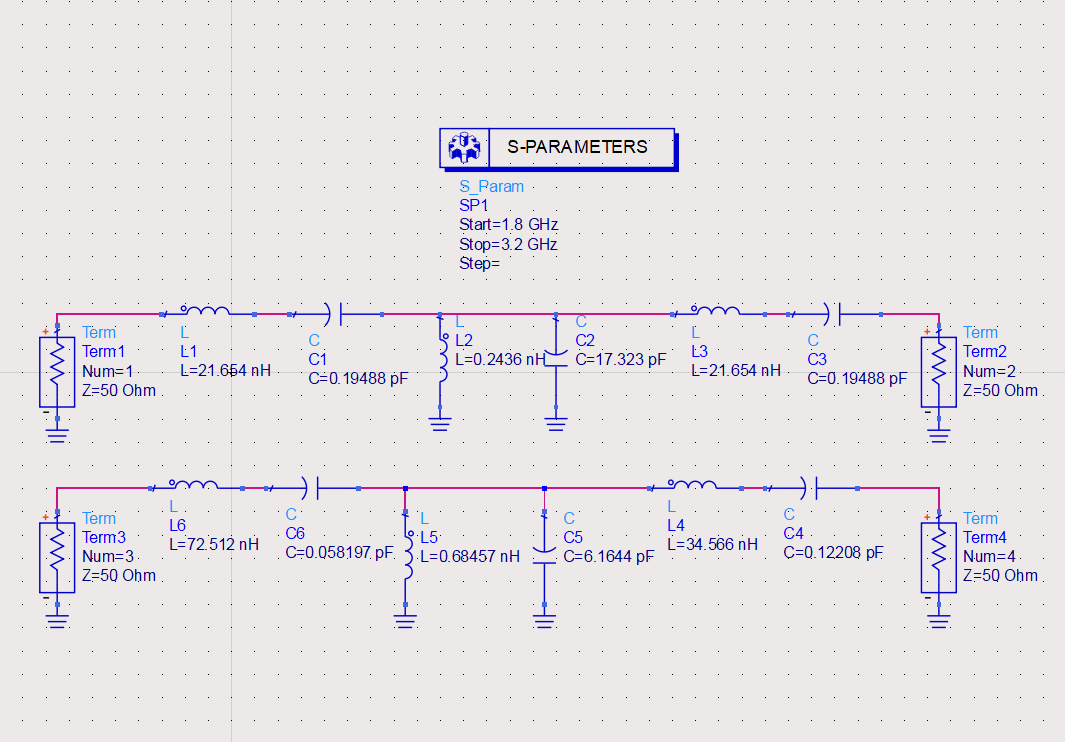
\includegraphics[scale=0.4]{images/butterworth_vs_chebyshev3pt0_schematic.png}
    \caption{Butterworth vs. 3 dB Chebyshev Schematic}
    \label{fig:20}
\end{figure}
\begin{figure}[h!]
    \centering
    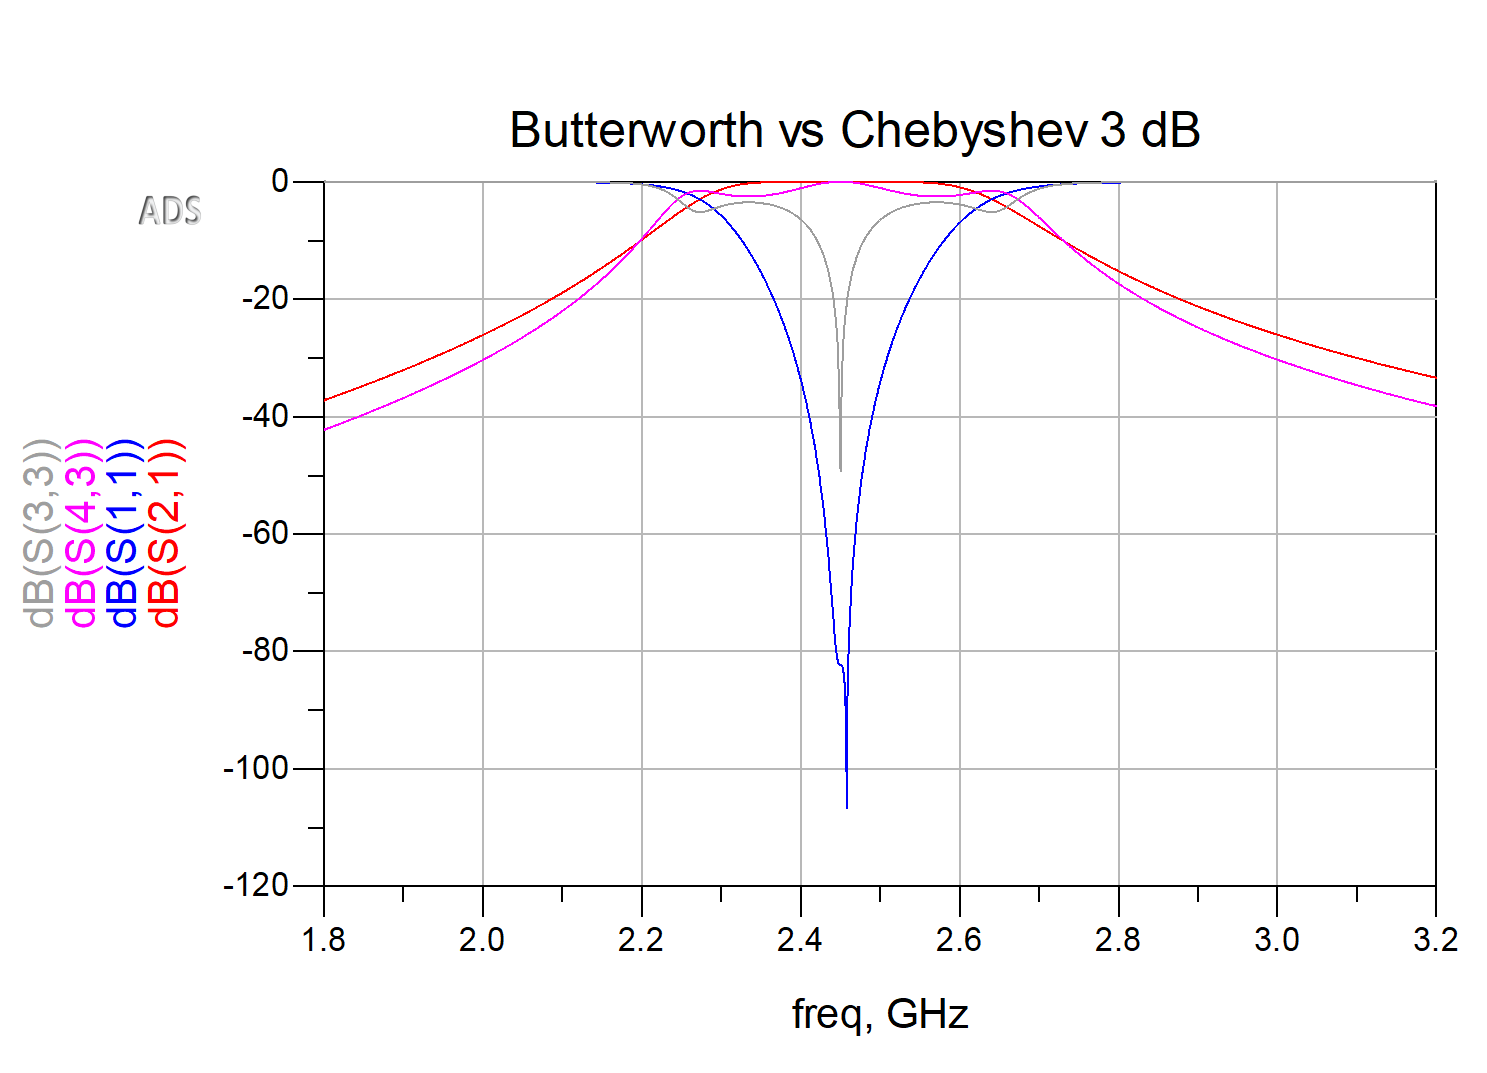
\includegraphics[scale=0.3]{images/butterworth_vs_chebyshev3pt0_plot.png}
    \caption{Butterworth vs. 3 dB Chebyshev Plot}
    \label{fig:21}
\end{figure}
\begin{figure}[h!]
    \centering
    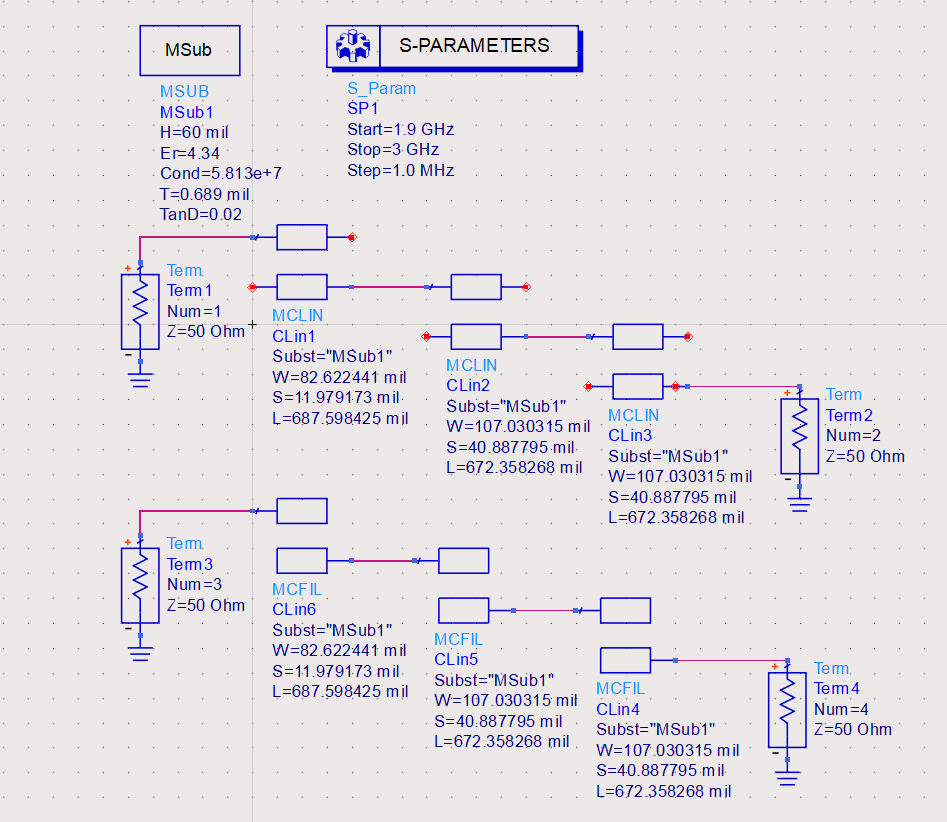
\includegraphics[scale=0.4]{images/mcfil_vs_mclin_schematic.png}
    \caption{MCLIN vs. MCFIL ADS Schematic}
    \label{fig:22}
\end{figure}
\begin{figure}[h!]
    \centering
    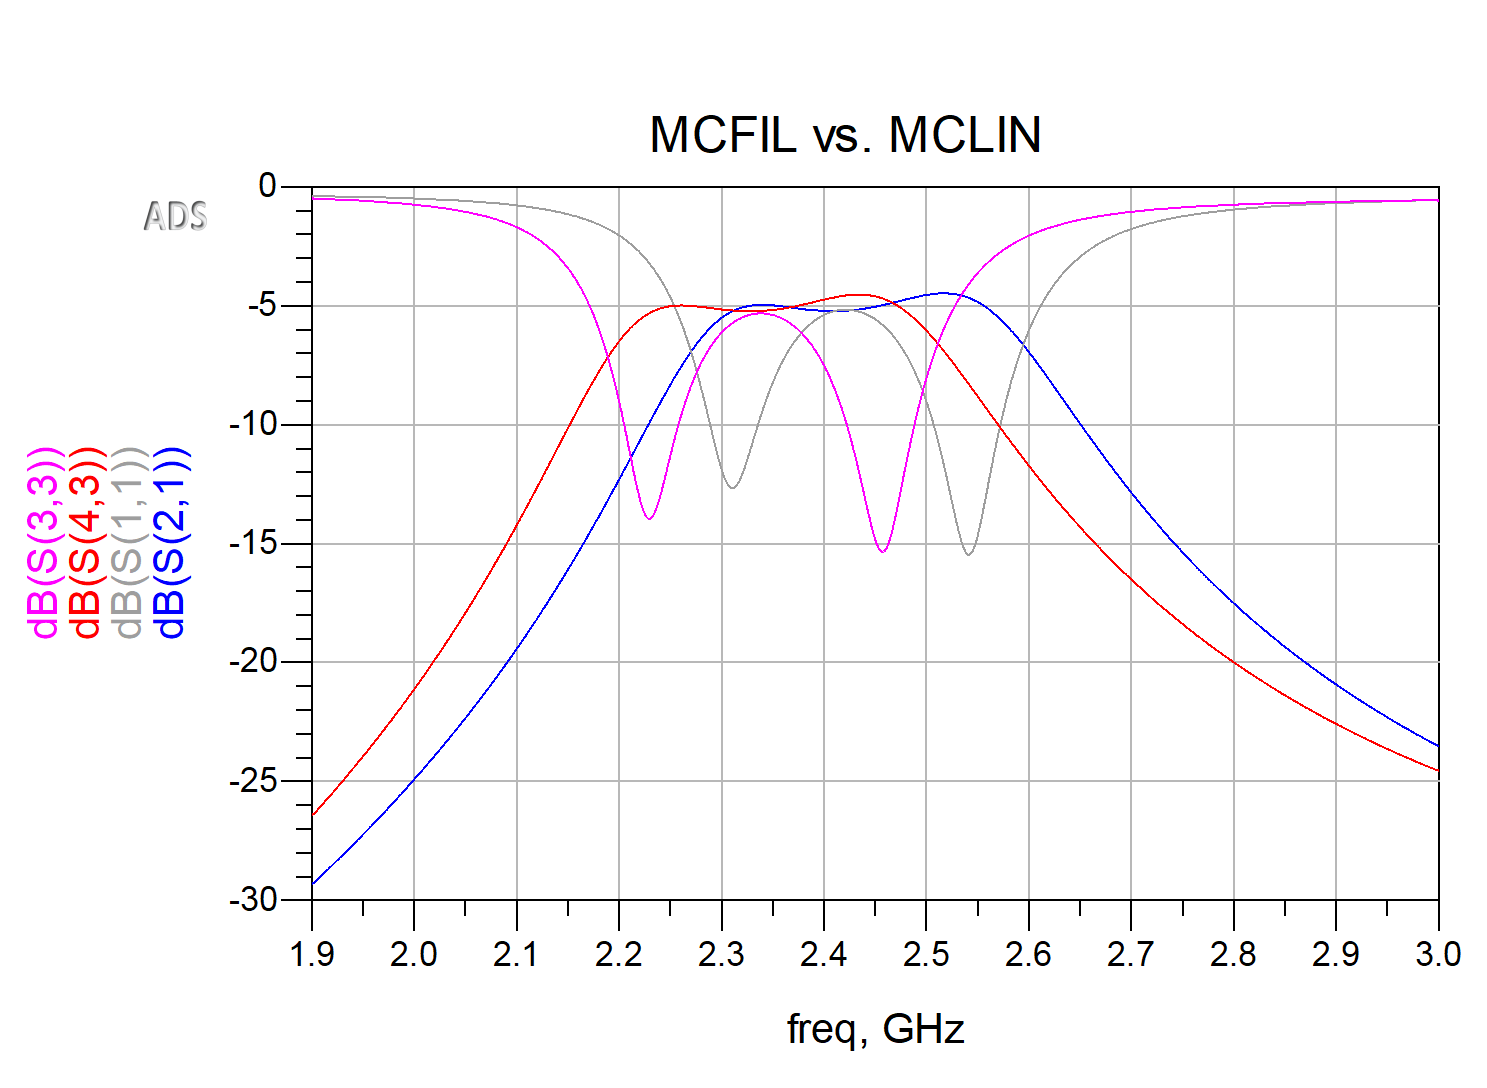
\includegraphics[scale=0.3]{images/mcfil_vs_mclin_plot.png}
    \caption{MCLIN vs. MCFIL ADS Plot}
    \label{fig:23}
\end{figure}

\begin{figure}[h!]
    \centering
    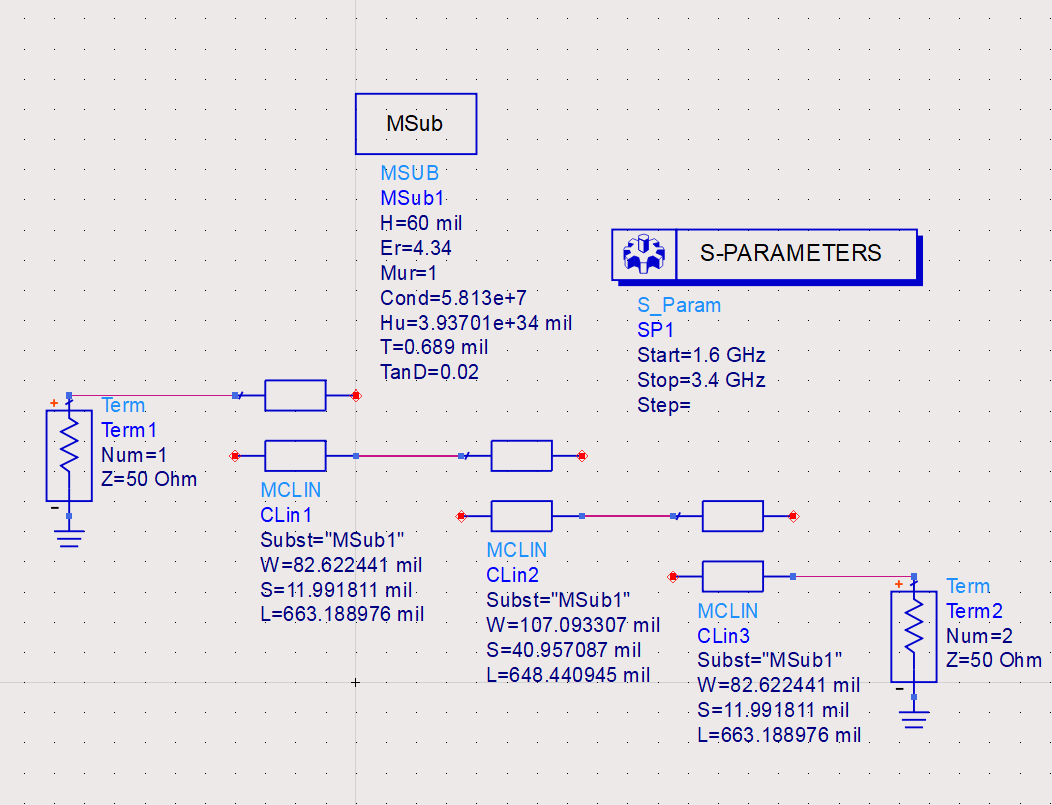
\includegraphics[scale=0.4]{images/my_filter_schematic.png}
    \caption{MCLIN Bandpass Filter Schematic}
    \label{fig:24}
\end{figure}
\begin{figure}[h!]
    \centering
    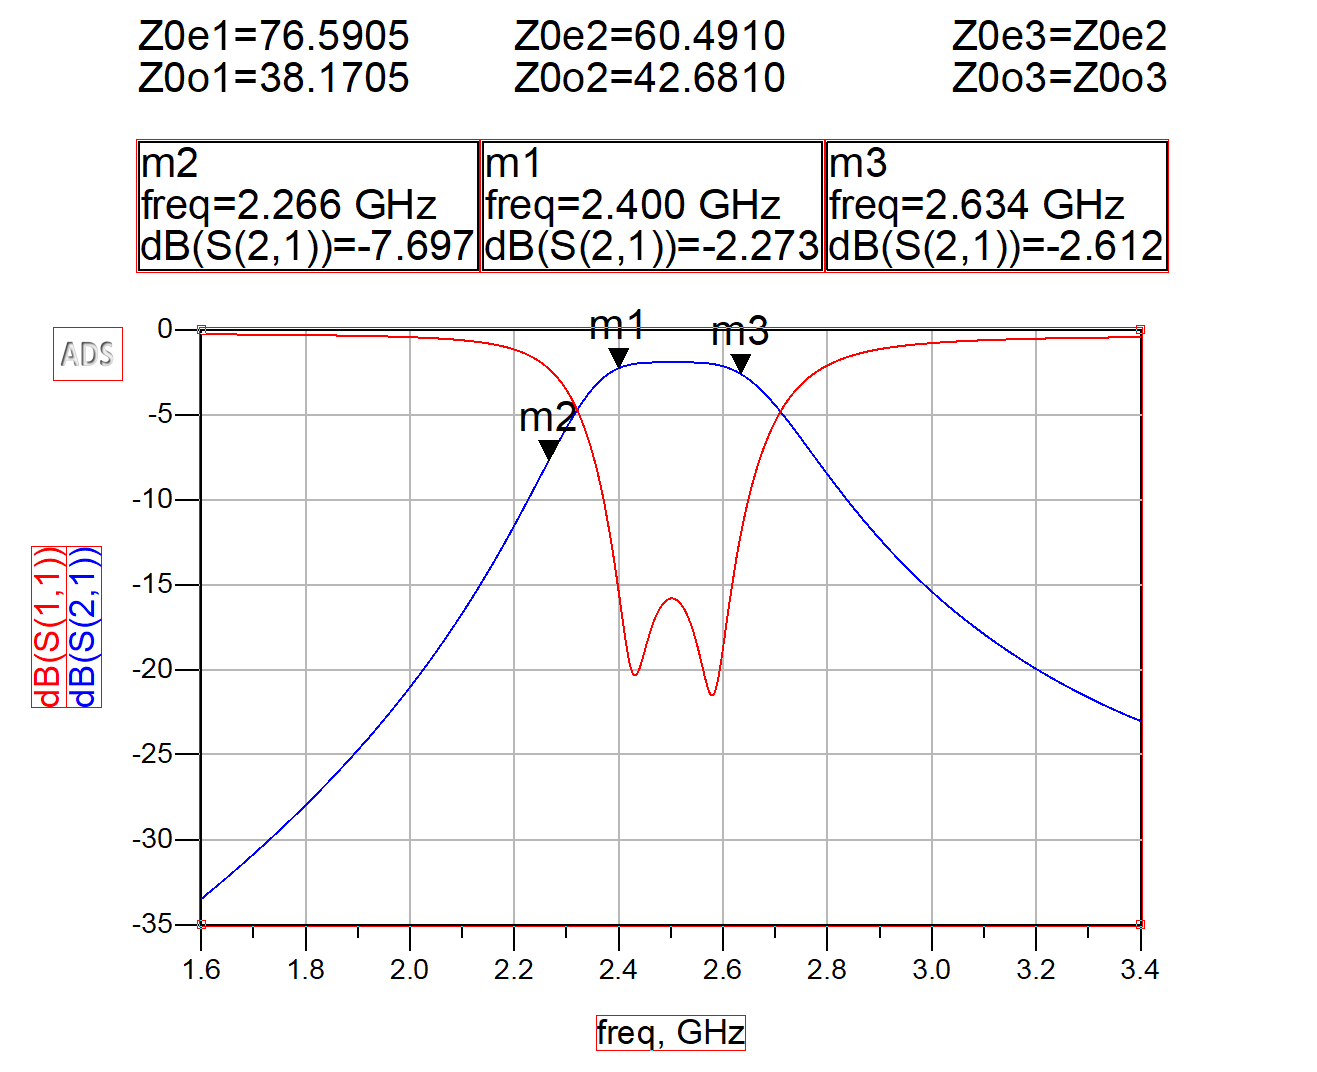
\includegraphics[scale=0.3]{images/my_filter_plot.png}
    \caption{MCLIN Bandpass Plot}
    \label{fig:25}
\end{figure}
\begin{figure}[h!]
    \centering
    \includegraphics[scale=0.075]{images/my_filter_fab.png}
    \caption{MCLIN Bandpass Filter}
    \label{fig:26}
\end{figure}

\clearpage
\printbibliography
\end{document}
